% REMEMBER: You must not plagiarise anything in your report. Be extremely careful.
\documentclass{l4proj}

    
%==============================================================================
% Put any additional packages here
% You can add any packages you want, as long as it does not alter
% the overall format (e.g. don't change the margins or the reference style).
%
\usepackage{pdfpages} % if you want to include a PDF for an ethics checklist, for example
%
%

\begin{document}

%==============================================================================
%% METADATA
\title{Predicting drugs that can cross the blood-brain barrier} 
\author{George Iniatis}
\date{April 1, 2022}

\maketitle

%==============================================================================
%% ABSTRACT
\begin{abstract}
\textbf{Background}: The blood-brain barrier (BBB) prevents the vast majority of all compounds from entering the brain, protecting it from diseases and infections. However, it can also prevent useful therapeutics combating brain or central nervous system (CNS) related diseases from reaching their target.

\textbf{Motivation}: Checking whether a specific drug or compound can penetrate the BBB with experimental trials is expensive, time consuming and highly inefficient. Therefore, a predictive system can be a highly valuable tool that can test thousands of drugs and compounds in an inexpensive, fast and efficient manner.

\textbf{Aims}: This project aimed to create a new curated data set and then using it train machine learning models that make use of a drug's or compound's chemical properties to predict whether it can penetrate the BBB or not.

\textbf{Methods}: Both classification and regression models were trained using subsets of a curated data set of 2396 publicly available drugs and compounds and 6 hydrogen-bonding chemical descriptors. The classification models were further improved through the addition of the available side effects and indications to the chemical descriptors. Unfortunately this could not be replicated for the case of the regression models due to the subset size. All models were checked for robustness and evaluated using dummy models and holdout test sets.

\textbf{Results}: Our best classification model with just chemical descriptors used as features was the Random Forest Classifier which achieved an F1 score of 0.8506, an Accuracy of 0.8116, a Recall score of 0.9250, a Precision score of 0.7872 and a Matthews Correlation Coefficient of 0.6145. Our best classification model with chemical descriptors and a selection of side effects and indications as features was again the Random Forest Classifier, which achieved an F1 score of 0.8642, an Accuracy of 0.8406, a Recall score of 0.8750, a Precision score of 0.8537 and a Matthews Correlation Coefficient of 0.6716. Our best regression model with chemical descriptors used as features was the Support Vector Regression model, which achieved an R2 score of 0.4746, and a Negated Mean Absolute Error of -0.3968. A Streamlit web application was then created to showcase all of our work.
\end{abstract}






%==============================================================================
%==============================================================================

% EDUCATION REUSE CONSENT FORM
% If you consent to your project being shown to future students for educational purposes
% then insert your name and the date below to  sign the education use form that appears in the front of the document. 
% You must explicitly give consent if you wish to do so.
% If you sign, your project may be included in the Hall of Fame if it scores particularly highly.
%
% Please note that you are under no obligation to sign 
% this declaration, but doing so would help future students.
%
%\def\consentname {My Name} % your full name
%\def\consentdate {20 March 2018} % the date you agree
%
\def\consentname {George Iniatis} % your full name
\def\consentdate {1 April 2022} % the date you agree
\educationalconsent



%==============================================================================
\tableofcontents

%==============================================================================
%% Notes on formatting
%==============================================================================
% The first page, abstract and table of contents are numbered using Roman numerals and are not
% included in the page count. 
%
% From now on pages are numbered
% using Arabic numerals. Therefore, immediately after the first call to \chapter we need the call
% \pagenumbering{arabic} and this should be called once only in the document. 
%
%
% The first Chapter should then be on page 1. 

% PAGE LIMITS
% You are allowed 40 pages for a 40 credit project and 30 pages for a 
% 20 credit report. 
% This includes everything numbered in Arabic numerals (excluding front matter) up
% to but *excluding the appendices and bibliography*.
%
% FORMATTING
% You must not alter text size (it is currently 10pt) or alter margins or spacing.
% Do not alter the bibliography style. 
%
%==================================================================================================================================
%
% IMPORTANT
% The chapter headings and structure here are **suggestions**. You don't have to follow this model if
% it doesn't fit your project. Every project should have an introduction and conclusion,
% however.  If in doubt, your supervisor can give you specific guidance; their view takes precedence over
% the structure suggested here.
%
%==================================================================================================================================
\chapter{Introduction}

% reset page numbering. Don't remove this!
\pagenumbering{arabic} 

%\footnote{Specifying an online resource like %\url{https://developer.android.com/studio}
%in a footnote sometimes makes more sense than %including it as a formal reference.}

%\todo{Remove everything above}

This chapter will introduce the project on a high level and examine its motivations and objectives.

\section{Motivation}
\label{sec:Motivation}

The blood-brain barrier (BBB) can have a complex medical definition. However, for the sake of simplicity and the purposes of this project, we can think of it as a semi-permeable membrane that only allows molecules that are small or fat-soluble to enter the brain, and by definition, the central nervous system (CNS), while preventing larger ones from gaining entry \citep{Woodruff2017}. This process is called passive diffusion, but it should also be noted that there are certain types of larger molecules, one of them being glucose, that can still enter the brain using different methods, such as through the usage of transport proteins \citep{Woodruff2017, Gao2017}.

Just as the skull and cerebrospinal fluid, the fluid surrounding the brain, protect it from physical damage, the blood-brain barrier protects it from internal threats, such as harmful toxins and pathogens, that can cause infections and diseases \citep{Woodruff2017}. This protective barrier prevents 98\% of compounds from entering the brain. However, this can also mean preventing useful drugs from reaching their target, and this can be especially important when trying to deliver life-saving medicine like chemotherapy agents to combat brain tumours \citep{Gao2017}.

Manually checking whether a drug can penetrate the blood-brain barrier or not using laboratory experiments is expensive, time-consuming and can only be done one drug at a time, making the whole process highly inefficient \citep{Singh2020}. On the other hand, a prediction system can test thousands of drugs quickly and cheaply and can be used effectively as an early screening process, leading to a better allocation of time and resources for manual checks by discovering those drugs or compounds worth checking in more detail.

\section{Objectives}
\label{sec:Objectives}

The project aimed to gather publicly available data on drugs known to cross into the brain and those that cannot and place them into a new curated data set and then using this new data set train multiple machine learning models that use a drug's or compound's chemical properties to predict whether it can pass into the brain or not. The models should then be evaluated and compared in terms of robustness and performance, and a rudimentary system using these models should be constructed.

\section{Outline}

The dissertation consists of 6 chapters, including this one, where each discusses and examines a different stage of the project's life-cycle.

\begin{itemize}
\item \textbf{Chapter 2 - Background} \\
Explores how other researchers have tackled the same problem and the valuable strategies, techniques, and knowledge discovered from their experiments.
\item \textbf{Chapter 3 - Requirements Analysis} \\
Discusses the high-level decisions made to narrow the scope of the project.
\item \textbf{Chapter 4 - Design \& Implementation} \\
Explores how the data set and various machine learning models
were created, using the decisions already discussed in Chapter 3.
\item \textbf{Chapter 5 - Results \& Evaluation} \\
Discusses data exploration findings and the predictive performances of our trained models.
\item \textbf{Chapter 6 - Conclusion} \\
Summarises the project and discusses valuable lessons learned and any possible future work that could potentially improve our findings. 
\end{itemize}
%==================================================================================================================================
\chapter{Background}
\label{ch:Background}

In this chapter we will explore how other researchers have tackled the same problem and the valuable strategies, techniques, and knowledge discovered from their experiments.

This background research was one of the first steps in the project's life-cycle and was instrumental in better understanding this previously unknown problem which included complex chemical and medical concepts, while also introducing us to key machine learning concepts and best practices.

Due to the important nature of the problem, as discussed in Section \ref{sec:Motivation}, there have been numerous attempts to construct classification and regression machine learning models using a variety of different methods, techniques, chemical properties and other characteristics that can be extracted from the drugs themselves, such as the drug's side effects and indications, what illness they treat. \citep{Singh2020,Saber2020,Zhao2007,Gao2017,Zhang2008}. 

 Classification models, being the ones that are more widely used, try to predict whether a particular compound or drug can pass the blood-brain barrier (BBB+) or not (BBB-), and Regression models try to predict the ratio between the concentration of a compound in the brain compared to the one in the blood. This ratio is called the Brain/Plasma ratio, but studies, more often than not, use its logarithmic version called logBB.

\section{Traditional Approach Utilising Chemical Descriptors}

The classic approach to solve the problem through the creation of classification models, as showcased by \citet{Singh2020}, and regression models, as showcased by \citet{Zhang2008}, was through the usage of special software that would use the SMILES notation of a drug or compound, that essentially describes its unique chemical structure, to produce thousands, if not more, chemical descriptors. Some of these special software included \citet{Molconn-Z}, \citet{MOE}, \citet{Dragon}, used by \citet{Zhang2008} and PaDEL-Descriptors \citep{Yap2011}, used by \citet{Singh2020}. Even if the descriptors with low predictive ability were removed, just as it was done in the case of \citet{Singh2020}, hundreds of descriptors would still be left. These descriptors would then be used to train the various models.

Both \citet{Singh2020} and \citet{Zhang2008} concluded that a 
consensus model would provide superior predictive ability than a single model. This is because a consensus model combines multiple models and therefore mitigates overfitting problems associated with a single model. However, it naturally requires more computational power.

\subsection{Applicability Domain}

\citet{Zhang2008} used a very interesting concept called applicability domain (AD) which essentially calculated the "Euclidean distance between each compound and its k-nearest neighbours" and compared it with a threshold, and if it exceeded that threshold, the prediction for that specific compound would not be made.
 
 However, a case could be made that this takes away from the aim of building a predictive system used to test existing but also new drugs, drugs that could potentially be vastly different from their predecessors, leading to a large euclidean distance.

\subsection{Pitfalls}

The main pitfall to this traditional approach was the usage of special software that produced a massive number of descriptors, slowing down the models' training times while providing minimal improvements to performance as discussed by \citet{Zhao2007}. Furthermore, the usage of these special, not widely available software would also make it very difficult for someone to use the created models to make predictions without having access to the specific one used to train them.

\subsection{Improvements}

\citet{Zhao2007} aimed to reduce the high number of descriptors needed to train classification models and using Algorithm Builder, a program developed by PharmaAlgorithms Inc, 19 molecular descriptors were calculated, showcased in Table \ref{tbl:Important_Chemical_Descriptors}. Small subsets of these descriptors were then used to train different models that achieve high predictive ability, effectively making the case that small numbers of descriptors are enough to create successful models.

The findings of \citet{Zhao2007} were further confirmed by \citet{Saber2020}, making use of the same data set and choosing a subset of 8 uncorrelated chemical descriptors from the 19 previously used (Labelled as 6, 7, 8, 10, 11, 12, 13 and 19 in Table \ref{tbl:Important_Chemical_Descriptors}). It again proved that highly predictive models could be constructed using a tiny number of descriptors. These highly efficient combinations were uncovered through the use of sequential feature selection (SFS) and genetic algorithms (GA), with the study concluding that GA is a more robust approach than SFS in choosing the most relevant chemical descriptors.

Choosing a small number of highly predictive and widely available chemical descriptors leads to improved model training times and predictive performances.

\begin{table}[!ht]
  \caption{Table taken from \citet{Zhao2007} showcasing the 19 different chemical descriptors calculated.}
  \label{tbl:Important_Chemical_Descriptors}
  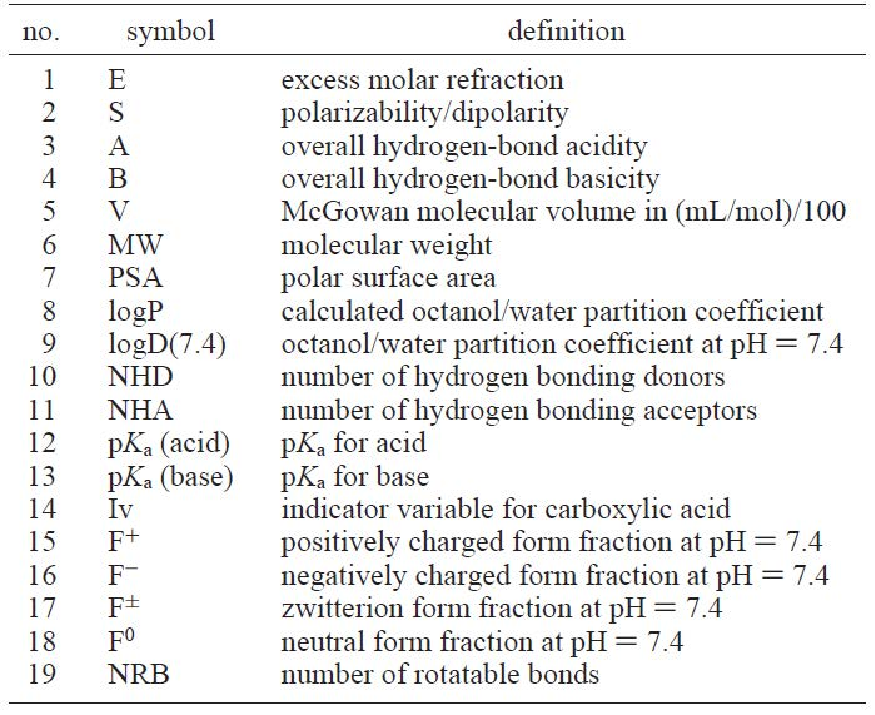
\includegraphics[width=0.55\linewidth]{images/Zhao_Table1.pdf}
\end{table}

\newpage

\section{Novel Approach Utilising Side Effects \& Indications}
\label{sec:Novel_Approach}

\citet{Gao2017} combined the usual approach of using the chemical characteristics of a drug or compound in order to predict its brain permeability with a new approach that makes use of their well-recorded side effects and indications found in the \citet{SIDER} database. 

As mentioned in Section \ref{sec:Motivation}, some larger molecules can pass into the brain using methods other than passive diffusion. These methods cannot be accurately described by the chemical characteristics of a drug or compound, but their recorded side effects and indications can capture them.

The side effects and indications were mapped to 43 subgroups, and SVM classification models were trained using multiple kernels. When both chemical descriptors and side effects and indications were available and combined, the models achieved significantly better performance than those based solely on the chemical descriptors, as showcased by Table \ref{tbl:Gao_Model_Comparison}

The study also used their created models on the \citet{SIDER} database and identified 110 drugs that can potentially penetrate the blood-brain barrier and 1018 that potentially cannot.

\begin{table}[!ht]
  \caption{Table taken from \citet{Gao2017} showcasing the different model metrics when utilising the chemical descriptors, the clinical phenotypes (meaning the side effects and indications), and a combination of the two. There seems to be a substantial increase in performance for the model utilising the combination of the two. *Prediction here means the average score achieved by cross-validation}
  \label{tbl:Gao_Model_Comparison}
  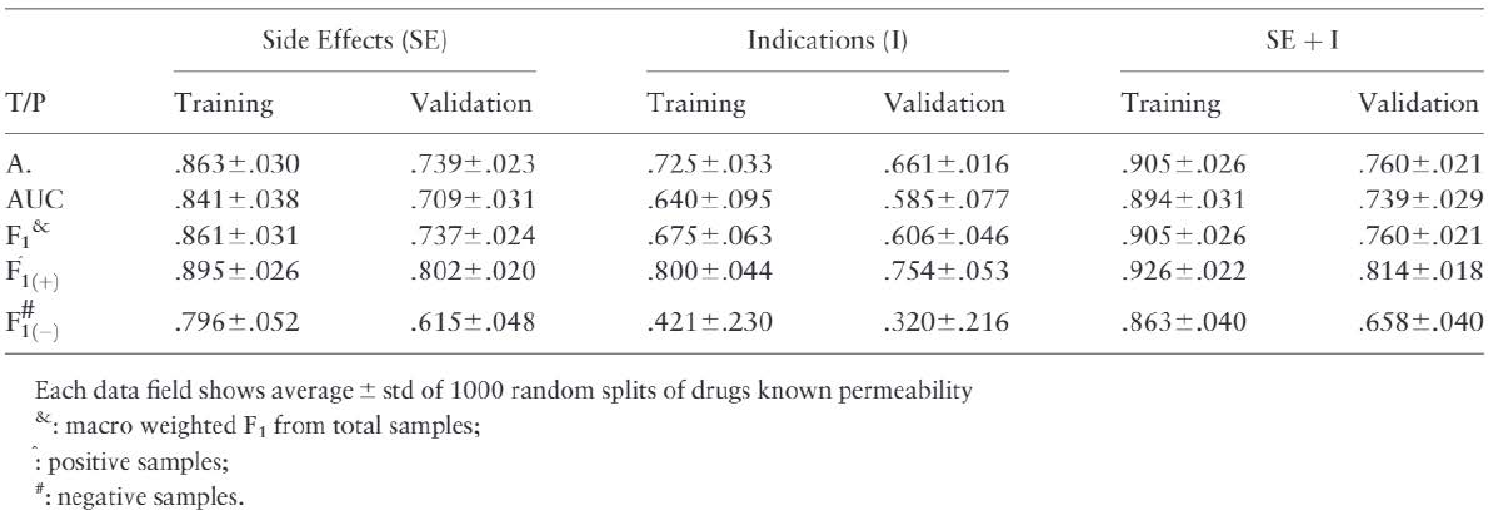
\includegraphics[width=1.0\linewidth]{images/Gao_Table_4.pdf}
\end{table}

\section{Important Chemical Descriptors}
\label{sec:Important_Chemical_Descriptors}

\citet{Zhang2008} after analysing the most frequent and vital descriptors, discovered that Polar surface area (PSA), Octanol/Water partition coefficient (logP) and the number of hydrogen bond donors and acceptor atoms were found to dominate the models. These findings were further confirmed and improved by the correlation study conducted by \citet{Zhao2007} which concluded that hydrogen-bonding properties (Labelled as 6-19 in Table \ref{tbl:Important_Chemical_Descriptors}) played a huge part in modelling brain permeability.

\citet{Singh2020} also illustrated the ranges that some of these crucial descriptors need to be within to successfully penetrate the blood-brain barrier and have an effect on the central nervous system (CNS), as showcased by Table \ref{tbl:Important_descriptors_ranges}.

However, it should be noted that even though CNS activity strongly implies BBB+, this cannot be said for the other way around, as BBB+ drugs and compounds can have no effect on the CNS.

\begin{table}[!ht]
  \caption{Table taken from \citet{Singh2020} showcasing the ranges that the most important chemical properties need to be within in order to be able to penetrate the blood-brain barrier and have an effect on the central nervous system}
  \label{tbl:Important_descriptors_ranges}
  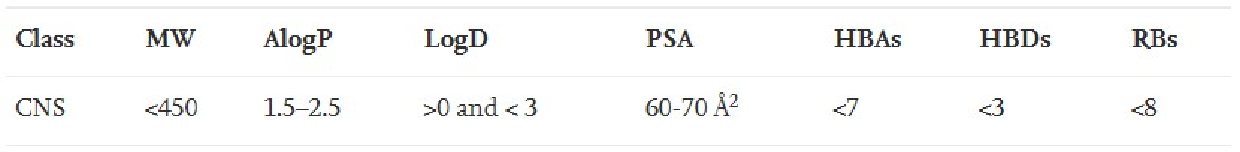
\includegraphics[width=1.0\linewidth]{images/Singh_Table1.pdf}
\end{table}

\section{Important Substructures}

\citet{Singh2020} discovered a list of corroborated substructures, as showcased in Table \ref{tbl:Substructure_Analysis}, that were more prevalent in BBB+ compounds and drugs. Even though this was something out of the scope for this project, future studies could possibly find this information helpful.

\begin{table}[!ht]
  \caption{Table taken from \citet{Singh2020} showcasing fragment occurrence in BBB+ and BBB- compounds.}
  \label{tbl:Substructure_Analysis}
  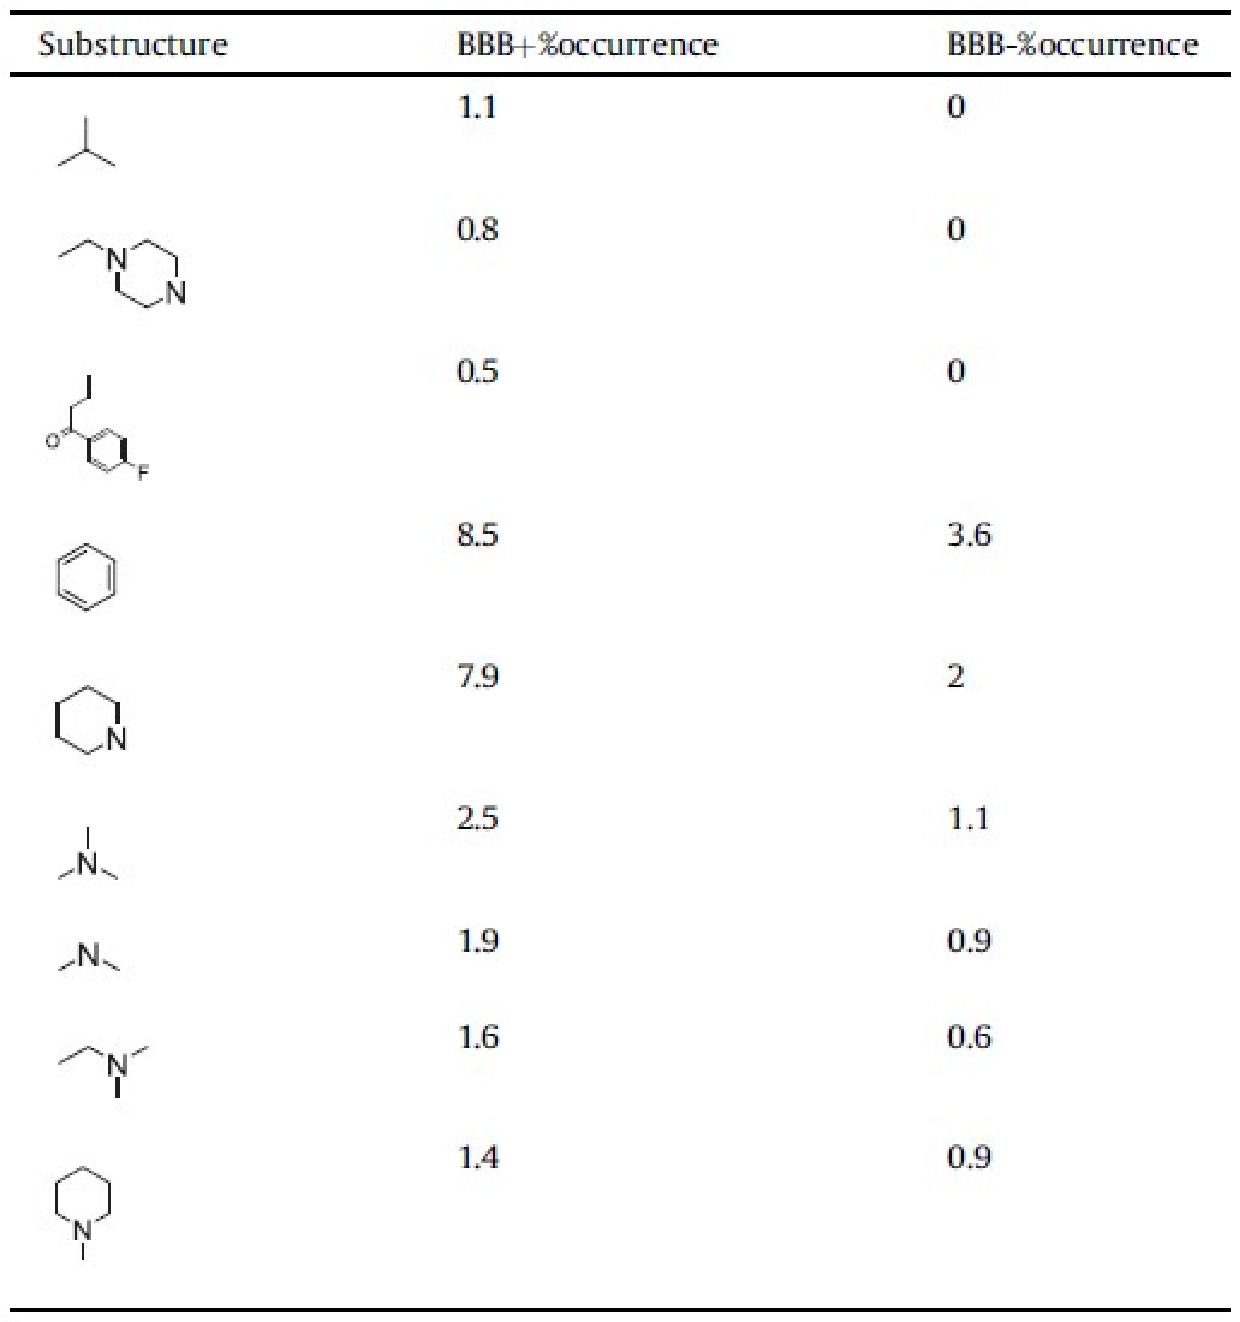
\includegraphics[width=0.45\linewidth]{images/Singh_Table13.pdf}
\end{table}

\section{Valuable Strategies \& Concepts Discovered}

All papers highlighted the importance of gathering as big a data set as possible, checking the robustness and statistical significance of models, and using holdout test sets to evaluate model predictive performance. 

The usage of small data sets leads to models not generalising effectively for unseen drugs or compounds outside their chemical space and thus making them unsuitable for high-throughput screening (HTS), which is the main objective of building such a system \citep{Singh2020}.

\citet{Zhang2008} also introduced us to the bias problem that can be caused by a class imbalance in the data set, which is often the case. This is due to the fact that most researchers are trying to discover drugs and compounds that can successfully penetrate the brain and not the other way around, naturally leading to a higher number of drugs and compounds that can enter the brain vs those that cannot, which then leads to a much higher predictive ability for the BBB+ class.


% Notes to add if needed
%\citet{Singh2020} trained Random Forest (RF), Multilayer Perceptron (MLP) and Sequential Minimal Optimisation (SMO) models.

%using two different Brain/Plasma ratio thresholds to determine whether a drug or compound can penetrate the blood-brain barrier or not.
%$$Threshold-1: Brain/Plasma \geq 0.6 \text{ as BBB+ and }Brain/Plasma < 0.6  \text{ as BBB-} $$
%$$Threshold-2: Brain/Plasma > 0.6 \text{ as BBB+ and } Brain/Plasma < 0.3 \text{ as BBB-} $$
%==================================================================================================================================
\chapter{Requirements Analysis}
\label{ch:Requirements_Analysis}

This chapter will discuss the high-level decisions made to narrow the scope of the project. 

Even though Section \ref{sec:Objectives} very clearly specified the objectives that this project aimed for, it gave us free rein on what methods and techniques we utilised to achieve them. 

These decisions, largely influenced by the background research found in Chapter \ref{ch:Background}, could be roughly split up into two distinct but interconnected sections that would determine the project's direction.

It should also be noted that some of these decisions, made early on in the project's life-cycle, were later revisited and updated accordingly, given our improved understanding of the problem and the methods we had used up to that point.

\section{Model Decisions}

The decisions that needed to be made for this section were the following:

\begin{itemize}
    \item
    Which machine learning library would we use.
    \item
    What type of models would we build.
    \item
    What metrics and methods would we use to evaluate the models' predictive performance.
    \item
    How would these models be optimised.
    \item
    How would we test these models for robustness.
    \item
    How would we make the models' predictions more interpretable.
    \item
    How would we present our findings.
\end{itemize}

\subsection{Machine Learning Library}

We decided to use scikit-learn \citep{scikit-learn} to build our models, as it is one of the best machine learning libraries with excellent documentation and tutorials available. 

\subsection{Model Types}
\label{subsec:Model_Types}

We had initially chosen to only build classification models but after going through the publicly available data sets, provided by the studies and papers we already discussed in Chapter \ref{ch:Background}, and noticing that the logBB values of some drugs and compounds were also provided in addition to their ability to penetrate the blood-brain barrier or not, we chose to build both classification and regression models.

We decided to use multiple metrics for both types of models to evaluate their performance. This was done as it is generally viewed as good practice and gives a more complete view of the models' performance and limitations. 

\subsection{Classification Metrics}

The classification models would be evaluated based on Precision, Recall, F1 Score, Accuracy and Matthews correlation coefficient (MCC). These metrics make use of the confusion matrix, which is a table, as shown in Figure \ref{fig:Confusion_Matrix}, that records the total number of true positives (TP) and negatives (TN) and false positives (FP) and negatives (FN).

Precision measures how many of the positive predictions made by the classifier were actually positive \citep{Precision}. It ranges from 0 to +1, with +1 being the best and 0 being the worst.

$$Precision =  \frac{TP}{TP + FP}$$

Recall, also known as Sensitivity, measures how many of the actual positives were labelled as positive by our classifier \citep{Recall}. It ranges from 0 to +1, with +1 being the best and 0 being the worst.
$$Recall = \frac{TP}{TP + FN}$$

F1 score is the harmonic mean of precision and recall \citep{F1}. Other variations exist where precision or recall can be given more or less weight. It ranges from 0 to +1, with +1 being the best and 0 being the worst.
$$F1 = \frac{2 * (precision * recall)}{precision + recall}$$
\label{itm:F1}

Accuracy measures the number of correct predictions made by the classifier \citep{Accuracy}. It ranges from 0 to +1, with +1 being the best and 0 being the worst.
$$Accuracy = \frac{TP + TN}{TP + TN + FP + FN} $$

Matthews correlation coefficient (MCC), also known as Phi coefficient, essentially calculates the correlation between the predicted and true values \citep{MCC}. It takes into account the whole confusion matrix and is generally thought of as a particularly useful metric, even when the classes are imbalanced.

MCC has a range of -1 to +1. A coefficient of +1 indicates a perfect relation between predicted and true values, 0 that our model is randomly guessing, and -1 an inverse relationship between predicted and true values \citep{MCC2}.

$$MCC = \frac{TP*TN - FP*FN}{\sqrt{(TP+FP)(TP+FN)(TN+FP)(TN+FN)}}$$

\newpage

\begin{figure}[!htb]
    \centering
    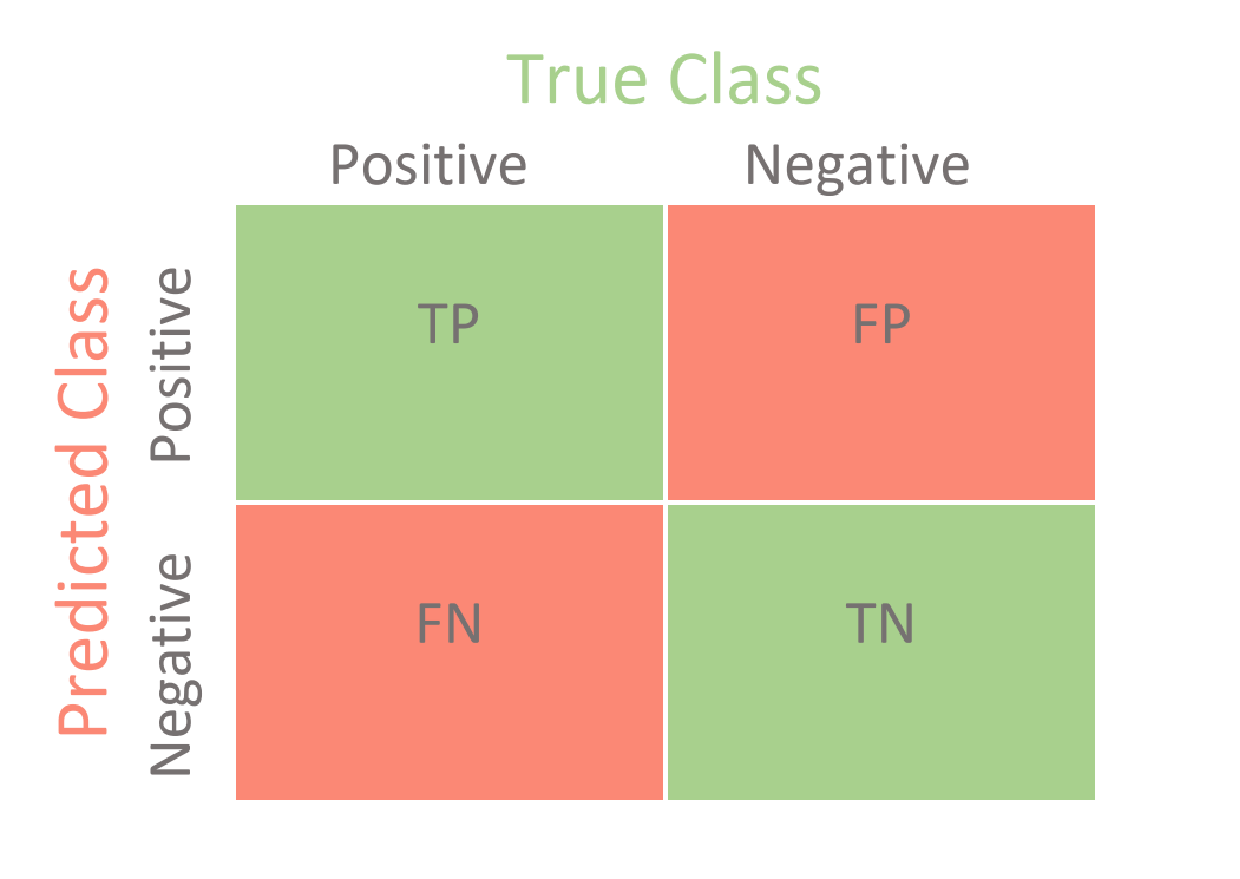
\includegraphics[width=0.8\linewidth]{images/TDS_Confusion_Matrix.pdf}    

    \caption{Figure taken from \citet{Confusion_Matrix} showcasing the confusion matrix for a binary classification problem.}

    \label{fig:Confusion_Matrix} 
\end{figure}

\subsection{Regression Metrics}

The regression models would be evaluated based on Negated Mean Absolute Error and R2 Score.

\newenvironment{conditions}
  {\par\vspace{\abovedisplayskip}\noindent\begin{tabular}{>{$}l<{$} @{${}={}$} l}}
  {\end{tabular}\par\vspace{\belowdisplayskip}}
  
The Mean Absolute Error (MAE) calculates exactly what its name suggests. It finds the absolute error, also known as the difference, between the predicted and the true value for all data points in a set, sums them up and then calculates their mean \citep{MAE}. It has a range of 0 to +$\infty$, with 0 being the best score.

The Negated Mean Absolute Error just adds a negative sign in front of MAE. It has a range of -$\infty$ to 0, with 0 again being the best score. We chose to use this variation so that all the metrics followed the same 'greater is better' principle, thus making their interpretation easier.

$$\text{Mean Absolute Error} (y,\hat{y}) = (\frac{1}{n})\sum_{i=1}^{n}\left | y_{i} - \hat{y}_{i} \right | $$

where: 
\begin{conditions}
n & number of samples\\
y & true values \\
\hat{y} & predicted values
\end{conditions}

The R2 score measures how good the regression line fits our data \citep{R2}. It compares the fit to a baseline model that essentially always predicts the mean of the true values \citep{R2_2}. Generally, it ranges from 0 to +1, with +1 being the best score, but it can also become negative, indicating a worse model.

$$\text{R2 Score} (y,\hat{y}) = 1 - (\frac{\sum_{i=1}^{n}(y_{i} - \hat{y}_{i})^2}{\sum_{i=1}^{n}(y_{i} - \bar{y})^2})$$

where: 
\begin{conditions}
n & number of samples\\
y & true values \\
\hat{y} & predicted values \\
\bar{y} & mean of true values
\end{conditions}

\subsection{Model Evaluation Methods}

We decided to use holdout test sets and dummy models to evaluate our models.

Holdout test sets are untouched subsets of the data, meaning they have not been used for training or validation purposes,  that are specifically employed to estimate the model's performance on unseen real-world data.

Dummy models usually predict the most frequent class in our data, in the case of classification models, and the mean of our labels, what we are trying to predict, in the case of regression models, although there are multiple variations \citep{DummyClassifier, DummyRegressor}. These would serve as the baselines for our models.

\subsection{Model Optimisation}
\label{subsec:Model_Optimisation}

The models' hyper-parameters would be tuned using scikit-learn's GridSearch function \citep{GridSearch} which makes use of cross-validation to optimise the models for a specific metric. 

GridSearch essentially splits the data provided into multiple training and validation subsets, with the default being five unless otherwise specified. Then it iteratively goes through the pairs of training and validation subsets, training the model on the training subset using a combination of its hyper-parameters and then uses the trained model to make predictions on the validation set and calculates a score. Once all the pairs have been used, it calculates the mean validation score, moves on to the following combination of hyper-parameters, and repeats the process until all the combinations have been exhausted.

The function can then return the scores for all combinations of hyper-parameters for inspection and the model with the best mean validation score, along with the hyper-parameters used to train it.

The metrics we chose to optimise our models were the F1 score for the classification models and the R2 score for the regression ones.

\subsection{Model Robustness}
\label{subsec:Robustness}

To check the robustness of the models, we would use scikit-learn's Permutation Test Score function. \citep{Permutation_Test_Score}. This process is also known as y-scrambling.

This is essentially a statistical hypothesis test with a null hypothesis stating that a statistical relationship does not exist between the features and label using our model and an alternative hypothesis stating that a statistical relationship does indeed exist using our model.

Again this function just as GridSearch, found in Subsection \ref{subsec:Model_Optimisation}, uses cross-validation. It iteratively goes through the pairs of training and validation sets and, for each permutation, randomly reorders the labels. Unless otherwise specified, this is repeated 100 times, removing any relationship between the features and the labels.

It returns a p-value which represents the probability that the model's predictions are just the result of random chance. The p-value is just the fraction of permutations that their mean validation score is better than the mean validation score obtained using the original data that correctly matches the features with their labels \citep{Permutation_Test_Score_Explanation}. Generally, if this p-value is less than or equal to 0.05, we assume that we have a statistically significant result and reject the null hypothesis.

\subsection{Model Interpretability}
\label{subsec:Interpretability}

Model interpretability was one of the last and most challenging questions we tackled. So we decided to try and make our models more interpretable to shine some light in their inner workings and instil some confidence in their predictions, or at the very least help whoever is using them understand what led to that prediction.

We decided to use \citet{ELI5} to examine the weights of the models' features and \citet{LIME} to explain how those features and their values led to a specific prediction.

\subsection{Presenting Findings}

The presentation of our findings was in flux until the very last stages of the project. We had previously discussed that, at the very least, we should produce a notebook or a simplistic web app. In the end, we decided to create a very simple \citet{Streamlit} web application that showcases the project's processes and the models produced.

\section{Data Set Decisions}
\label{sec:Dataset_Decisions}

The decisions that needed to be made for this category were the following:

\begin{itemize}
    \item
    What would we use as our label.
    \item
    What chemical descriptors would we use.
    \item
    Could we make use of other drug characteristics.
    \item
    How would the data set be built, and more specifically, what sources and methods would we use to create it.
\end{itemize}

\subsection{Labels}
\label{subsec:Labels}

For our classification models, the label would be whether a drug or compound can penetrate the blood-brain barrier or not, designated by a 1 and a 0, respectively, and for our regression models, the label would be the logBB value.

\subsection{Chemical Descriptors}
\label{subsec:Chemical_Descriptors}

After concluding our background research, discussed in Chapter \ref{ch:Background}, we had decided to use a tiny number of widely available chemical descriptors, specifically the same ones used by \citet{Saber2020}. 

Naturally, one of the world's largest and freely accessible databases of chemical information, \citet{PubChem}, was an excellent fit for our needs. However, we early on noticed that pKa (strongest base) and pKa (strongest acid) were not available, two of the eight chemical descriptors we wanted to use, and instead, we just had access to the pKa. So we made the decision to make use of this pKa descriptor, but we then observed that for the vast majority of drugs and compounds, this chemical descriptor was unavailable, so we finally settled on outright removing it from the data set altogether, reducing the number of chemical descriptors from 8 to 6.

The chemical descriptors we ended up using were:

\begin{itemize}
    \item
    Molecular weight (MW)
    \item
    Topological polar surface area (TPSA)
    \item
    Octanol-water partition coefficient (XLogP)
    \item
    Number of hydrogen-bond donors (NHD)
    \item
    Number of hydrogen-bond acceptors (NHA)
    \item
   Number of rotatable bonds (NRB)
\end{itemize}

\subsection{Other Characteristics}
\label{subsec:Other_Characteristics}

Inspired by the novel approach used by \citet{Gao2017} to solve the problem, as discussed in Section \ref{sec:Novel_Approach}, we also decided to make use of the recorded side effects and indications of drugs and compounds stored in the \citet{SIDER} database, to test whether the addition to the chemical descriptors improved the predictive performance of our models or not.

Side effects and indications pointing to central nervous system (CNS) issues should act as powerful indicators that a drug or compound can successfully penetrate the blood-brain barrier. However, just as it was already mentioned in Section \ref{sec:Important_Chemical_Descriptors} BBB+ drugs and compounds can have no effect on the CNS, making it harder to detect blood-brain barrier penetration solely through the usage of side effects and indications as features. 

\subsection{Data Set Sources}

To create our data set, we decided to combine the publicly available data sets already provided by the studies and papers we previously discussed in Chapter \ref{ch:Background} and augment them to suit our own needs. 

As mentioned in Subsections \ref{subsec:Chemical_Descriptors} and \ref{subsec:Other_Characteristics} we would make use of the \citet{PubChem} database to retrieve the chemical descriptors for each drug and compound and the \citet{SIDER} database to retrieve the side effects and indications.

We also aimed to further expand the size of the data set using straightforward text mining techniques on google searches about blood-brain permeability. Unfortunately, this was proven to be noisy and unreliable. However, the techniques and methods developed were easily repurposed on searches performed on medical APIs, like \citet{PubMedAPI} and \citet{SpringerAPI}, which proved to be much more reliable.



%==================================================================================================================================
\chapter{Design \& Implementation}

This chapter will explore how the data set, and various machine learning models were created, using the decisions already discussed in Chapter \ref{ch:Requirements_Analysis}.

\section{Data Set Creation Process}

Taking into consideration all the data set decisions discussed in Section \ref{sec:Dataset_Decisions}, the data set creation process was split up into sequential steps.

\subsection{Combining Publicly Available Data Sets}

To create our data set, we started by combining the publicly available data sets provided by \citet{Singh2020, Zhang2008, Gao2017, Zhang2008}. All columns were removed except the ones with the SMILES notation, drug or compound name, experimental logBB value and blood-brain barrier permeability. We felt that this was the most appropriate strategy as all data sets used a vast array of chemical descriptors from different sources. Furthermore, this would allow us to retain the most essential information that we could then build upon.

Each academic paper's Digital Object Identifier (DOI) was provided as the source for compounds and drugs. When it was not available, either a link to \citet{PubMed} or \citet{PubMed_Central} was provided as the source.

It should also be noted that when the experimental logBB was available, BBB permeability was recalculated using the thresholds suggested by \citet{Li2005}:

$$ BBB+ \text{ if } LogBB >= -1 $$
$$ BBB- \text{ if } LogBB < -1  $$

Given that the vast majority of the data set was created using the process discussed above, its quality is as good or bad as those data sets it has built upon.

\subsection{Automated Google Searches}

In an effort to expand our data set, we initially decided to perform some basic text mining using automated google searches, using \citet{Google_Package}, querying about specific drugs and compounds not present in our data set and their relation to the blood-brain barrier.

Our strategy was to gather the first 10 URLs returned from our google search and their HTML contents, and then using regular expressions, try to find matches for our query, hopefully leading to an apparent relationship between our specific drug or compound and the blood-brain barrier. These matches and their associated URLs were then loaded onto excel files and manually verified or rejected. Unfortunately, this strategy was proven to be too targeted and ineffective, returning completely irrelevant results most of the time.

Learning from our experience and discovering a class imbalance heavily tilting towards BBB+ drugs and compounds in our data set, we decided to broaden our search to try and reduce this imbalance, querying about drugs and compounds unable to cross the blood-brain barrier.

We followed the same process as before, but this time collecting as many URLs as we could before getting a "429: Too many requests error" and using multiple variations of queries and regular expressions, as showcased in Listing \ref{lst:Queries}. Unfortunately, this strategy was also proven ineffective, returning results from online forums and sites clearly having nothing to do with peer-reviewed medical or chemical information. 
Even though we had collected some usable results from these strategies, we decided not to use them as someone could argue that they are incredibly unreliable and noisy. Discussion on how to overcome these shortcomings led us to the discovery of the medical APIs explored in the next section.

\begin{lstlisting}[language=python, label={lst:Queries}, caption={A small sample of the list of queries and regular expressions used in an effort to expand our data set using Google Searches.}]
    queries_and_regular_expressions = [

    ["\"not able to cross the blood brain barrier\"", ".*was not able to cross the blood.brain barrier.*"],
    ["\"not able to cross the bbb\"", ".*was not able to cross the bbb.*"],
    ["\"not able to penetrate the blood brain barrier\"", ".*was not able to penetrate the blood.brain barrier.*"],
    ["\"not able to penetrate the bbb\"", ".*was not able to not penetrate the bbb.*"],
    ["\"not able to pass through the blood brain barrier\"", ".*was not able to pass through the blood.brain barrier.*"],
    ["\"not able to path through the bbb\"", ".*was not able tp pass through the bbb.*"],
    ["\"not able to get through the blood brain barrier\"", ".*was not able to get through the blood.brain barrier.*"],
    ["\"not able to get through the bbb\"", ".*was not able to get through the bbb.*"]
    
    ]
\end{lstlisting}

\subsection{Medical APIs}

\citet{PubMedAPI} was used to get abstracts from \citet{PubMed} and academic papers from \citet{PubMed_Central} that matched multiple queries about drugs and compounds unable to penetrate the blood-brain barrier.

The various paragraphs of the abstracts and academic papers were extracted using XML parsing, and then, just as before, regular expressions were used to find matches based on our query. Finally, the matches were again loaded into excel files and manually verified.

\citet{PubMed} searches produced 15 usable drugs and compounds, 14 being BBB- and 1 surprisingly being BBB+, from 35 matches.

\citet{PubMed_Central} searches produced 91 usable drugs and compounds, with all being BBB-, from 361 matches.

\citet{SpringerAPI} was used to get abstracts, articles and journals and then the same process was used just as in the case above.

Springer Meta V2 searches allowed us to access the abstracts of articles and journals not open to the public and produced 42 usable drugs and compounds, with 41 being BBB- and 1 being BBB+, from 108 matches.

Springer Open access searches allowed us to access the publicly available full-text content of articles and journals and produced 109 usable drugs and compounds, with 106 being BBB- and 3 being BBB+, from 491 matches.

As mentioned above, the matches returned by the API searches had to be manually verified, and it should be mentioned that any human validated data is bound to have at least a few errors.

\subsection{Retrieving Chemical Descriptors, Side Effects \& Indications}

Once we had gathered all the drugs and compounds from the publicly available data sets and our API searches, \citet{PubChemAPI} was used to retrieve the chemical descriptors, already mentioned in Subsection \ref{subsec:Chemical_Descriptors}, as well as some other helpful information such as the PubChem CID, the unique identifier for each compound in the \citet{PubChem} database, the synonyms associated for each compound and its most common name, which was essentially the first synonym available. Even though the name of the compound was supplied in most of the cases by the data sets we had combined, we felt that it would make things easier down the road, and for anyone in the future that might utilise this work, if we used replaced it with the one in the PubChem database. 

We mainly used the SMILES notation of each drug or compound to search the PubChem database for a match to accomplish this task. If the SMILES notation was unavailable, we used the drug or compound name to search for a match. Naturally, we discovered that using the drug or compound name was less effective in getting a match from the database than the SMILES format, as the latter is unique for each drug or compound, whereas multiple drugs or compounds can use the same name, which can lead to confusion.

It should also be noted that some drugs and compounds do not have a name or any synonyms associated with them.

Once the synonyms were retrieved for a specific drug or compound, they were looked up in the \citet{SIDER} database. If a synonym was found in the SIDER database, we then retrieved the SIDER CID and the associated side effects and indications. 

SIDER offered two types of labels for side effects and indications, Lowest Level Terms (LLTs), taken directly from the official description of drugs, and Preferred Terms (PTs), which simplify multiple LLTs. We decided to use the PT side effects and indications since they condensed multiple LLTs.

\subsection{Final Adjustments}

Duplicates, drugs and compounds that could not be discovered and those without all chemical descriptors available were removed. This process decreased the size of the data set from 3748 drugs and compounds to 2396, with 1751 being BBB+ and 645 being BBB-. The data set was then finally sorted by drug name.

Table \ref{tbl:Dataset} showcases the first 10 rows of the final version of the data set.

\begin{table}[ht!]
  \caption{The first 10 rows of our finalised data set.}
  \label{tbl:Dataset}
  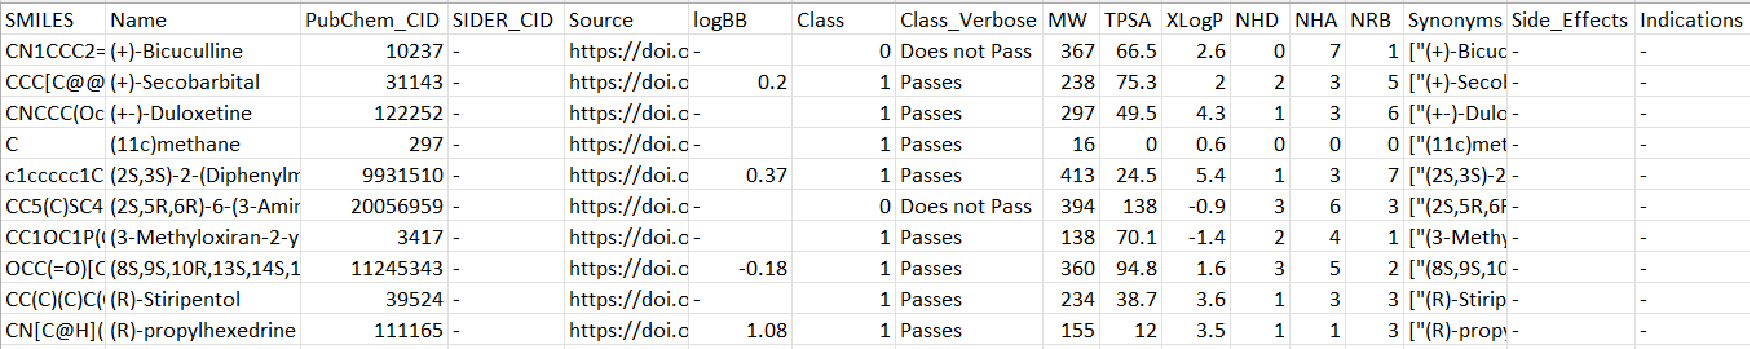
\includegraphics[width=1.0\linewidth]{images/Dataset.pdf}
\end{table}

\section{Model Training \& Testing Process}

Our training and testing process was straightforward and used consistently for both classification and regression models.

We would first create a pipeline \citep{Pipeline} containing a model and a standard scaler \citep{StandardScaler}. Pipelines simplify our workflow by stacking several pre-processing steps that are applied to our data before they are passed to a chosen model as features. In our case, we are just using a standard scaler as a pre-processing step that normalises our features by "removing the mean and scaling to unit variance".

We would then pass this pipeline to GridSearch \citep{GridSearch} as the estimator along with the specific model parameters we wanted to tune, the metrics we wanted to be returned, the metric we wanted to optimise for and the number of cross-validation folds. This process is showcased by Figure \ref{fig:Optimisation} to make things clearer.

All models were optimised using a 10-fold cross-validation GridSearch except in the case of the dummy classifier, dummy regressor and linear regression models.

Once optimised, the models were then tested for robustness, using permutation testing as already discussed in \ref{subsec:Robustness}, and used to make predictions on their respective test set.

\begin{figure}[htb]
    \centering
    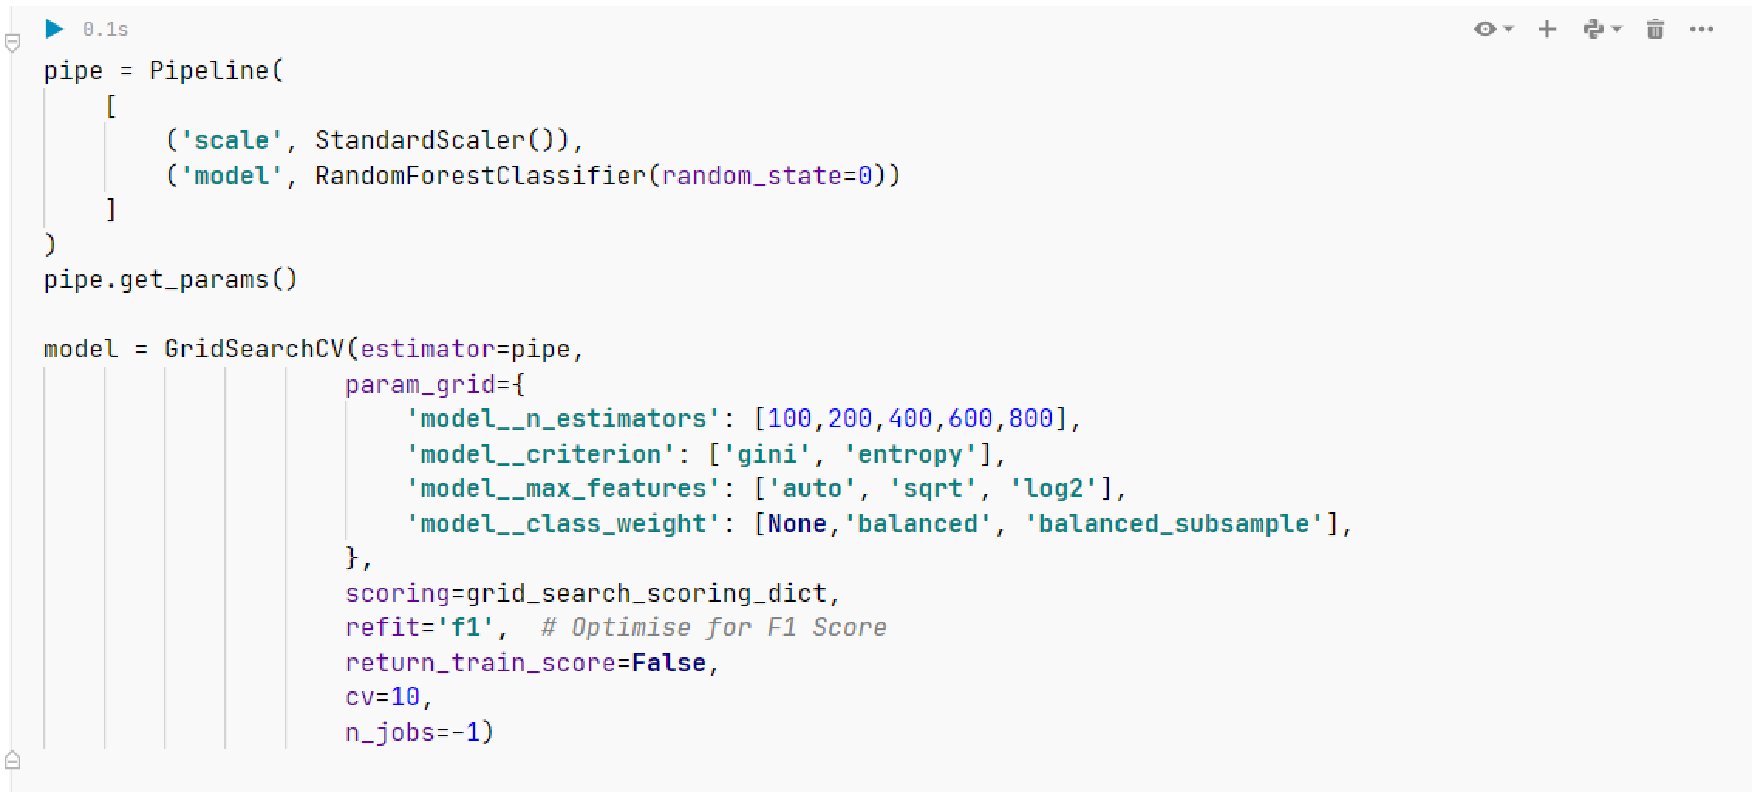
\includegraphics[width=1.0\linewidth]{images/Optimisation.pdf}    
    \caption{The optimisation process used for the majority of our models, showcased with a Random Forest Classifier.}

    \label{fig:Optimisation} 
\end{figure}

\subsection{Classification Models}
\label{subsec:Classification_Models}

Classification models were split up into two categories, one using just the chemical descriptors as features and the other using the chemical descriptors and a selection of one-hot encoded side effects and indications as features.

A selection was used instead of every single side effect and indication supplied by \citet{SIDER} to not only improve the training times of our models but to also potentially discover which side effects and indications play the most critical role in deciding blood-brain barrier permeability. To achieve this, we decided to use scikit-learn's recursive feature elimination with cross-validation (RFECV) function \citep{RFECV} which does exactly what it suggests, with a random forest classifier, optimising for F1 score, and a 10-fold cross-validation. As a result, RFECV managed to reduce our features from 4353 to 217, keeping all 6 chemical descriptors, 196 of the side effects and 15 of the indications.

We decided to split our classification models into two separate categories because we were interested in discovering whether the addition of side effects and indications to the chemical descriptors improved their predictive performance. Therefore, we needed a common holdout test set to achieve this.

This holdout test set was a 20\%  stratified split of the 345 drugs and compounds that had chemical descriptors, side effects and indications available (199 BBB+, 146 BBB-), produced with scikit-learn's Train Test Split function \citep{TrainTestSplit}. 

The training sets for both categories excluded the drugs and compounds present in the test set, with the first category making use of the whole data set, while the second one used the subset of drugs and compounds having chemical descriptors, side effects and indications available.

Finally, the classification models we decided to train for both categories were:
\begin{itemize}
    \item 
    Dummy Classifier
    \item 
    Logistic Regression
    \item 
    Support Vector Classifier
    \item 
    K-Nearest Neighbour Classifier
    \item 
    Random Forest Classifier
    \item 
    Decision Tree Classifier
    \item 
    Stochastic Gradient Descent Classifier
\end{itemize}

\subsection{Regression Models}

Regression models were solely trained using chemical descriptors as there were not enough drugs and compounds with logBB values available and chemical descriptors, side effects and indications to split them into two categories just as it was done in the case of the classification models.

The training and test sets were again produced using scikit-learn's Train Test Split function \citep{TrainTestSplit}. The holdout test set was a 20\% stratified split of the 401 drugs and compounds that had logBB values available (360 BBB+, 41 BBB-). The remaining 80\% was used as the training set.

Finally the regression models we decided to train were:
\begin{itemize}
    \item 
    Dummy Regressor
    \item 
    Linear Regression
    \item 
    Support Vector Regression
    \item 
    K-Nearest Neighbour Regressor
    \item 
    Random Forest Regressor
    \item 
    Decision Tree Regressor
    \item 
    Stochastic Gradient Descent Regressor
\end{itemize}


\section{Streamlit Web App}

The web app was created in the final weeks of the project to present a synopsis of our work and primarily showcase our models and to allow users to make predictions with them. A strong emphasis was also placed on model interpretability, helping users understand what led to a specific prediction by a model, which was already briefly discussed in Subsection \ref{subsec:Interpretability}. However, it should be noted that these interpretability tools are not available for all models.

Figure \ref{fig:Streamlit} showcases a prediction made by our trained Random Forest Classifier using our web application, and the interpretability tools, which a user can use to try and understand the model's prediction.

\href{https://share.streamlit.io/georgeiniatis/blood_brain_barrier_drug_prediction/main/Streamlit_App/app.py}{\textbf{You can access the web application using this link}}

\begin{figure}[htb]
    \centering
    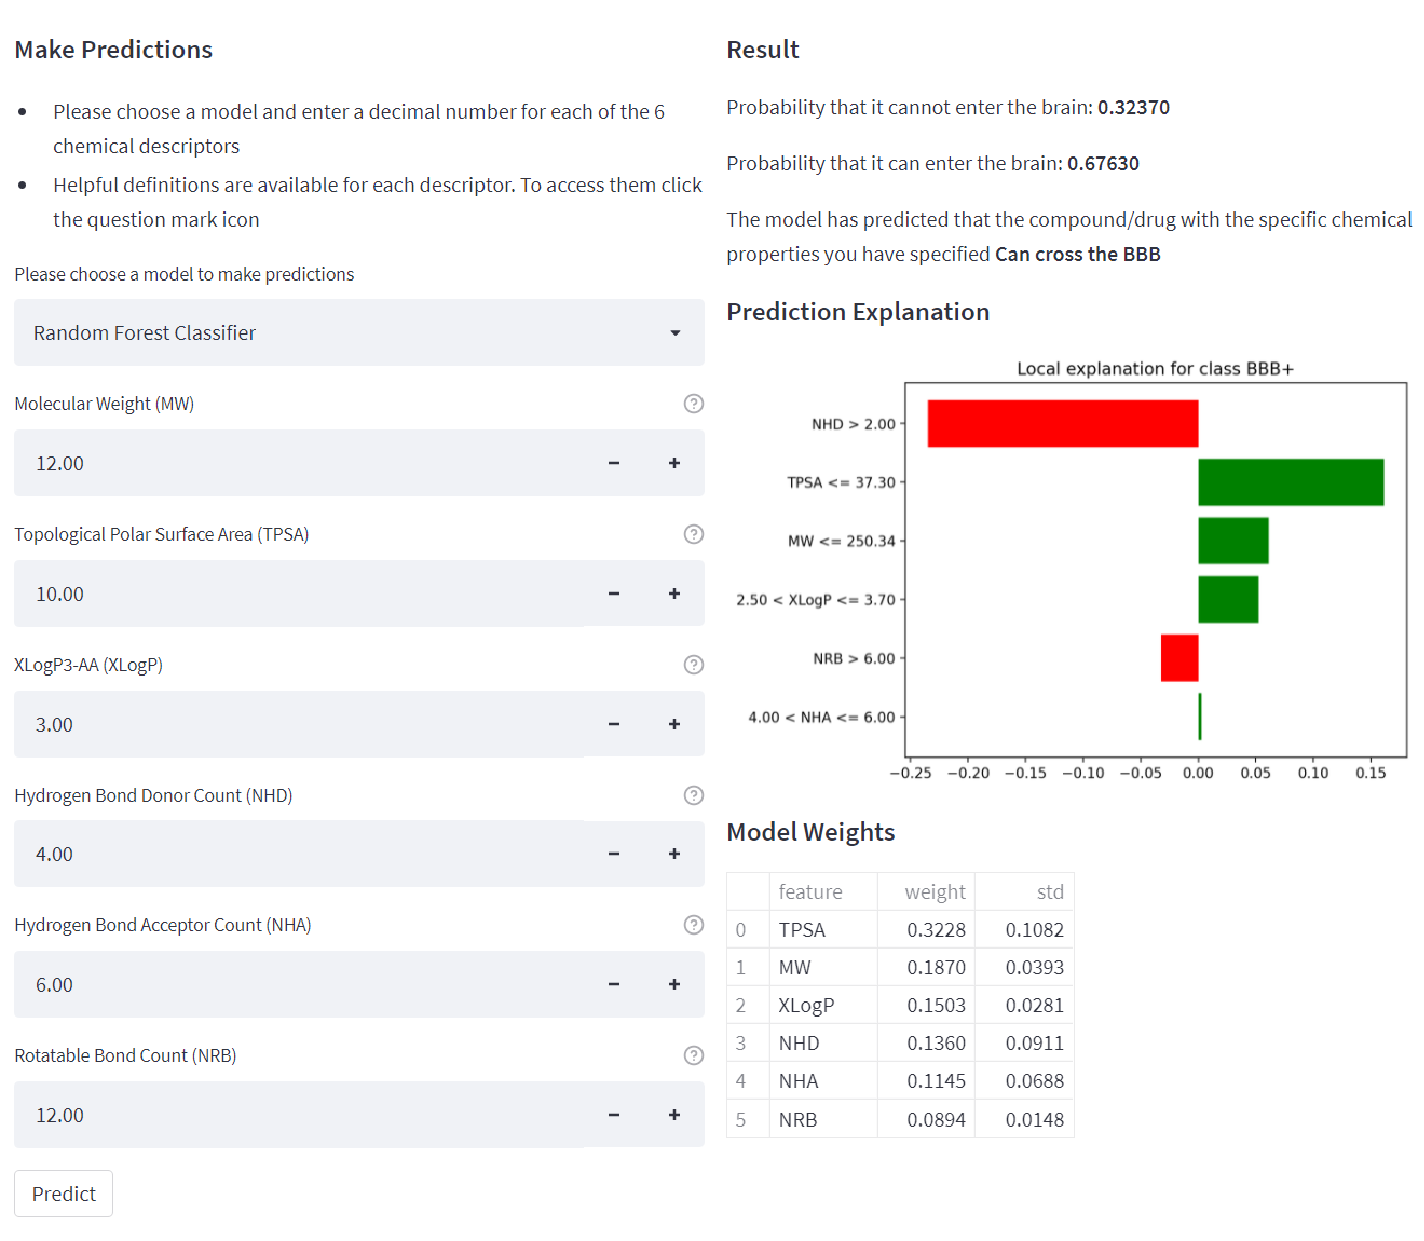
\includegraphics[width=0.8\linewidth]{images/Streamlit.pdf}    
    \caption{Our trained Random Forest Classifier used to make a prediction in our Streamlit Web App.}

    \label{fig:Streamlit} 
\end{figure}


 



%==================================================================================================================================
\chapter{Results \& Evaluation} 

%How good is your solution? How well did you solve the general %problem, and what evidence do you have to support that?

%\section{Guidance}
%\begin{itemize}
%    \item
%        Ask specific questions that address the general problem.
%    \item
%        Answer them with precise evidence (graphs, numbers, %statistical
%        analysis, qualitative analysis).
%    \item
%        Be fair and be scientific.
%    \item
%        The key thing is to show that you know how to evaluate your %work, not
%        that your work is the most amazing product ever.
%\end{itemize}

This chapter will discuss data exploration findings and the predictive performances of our trained models.

\section{Data Exploration}

After creating our data set, we wanted to explore our classes' spread and the distributions of the chemical descriptors. This section also discusses the essential side effects and indications discovered.

\subsection{Principal Component Analysis (PCA)}

Principal component analysis is a dimensionality reduction method used to project data in a lower-dimensional space \citep{PCA}. We used it to project our chemical descriptor data for all drugs and compounds into a two-dimensional space in order to plot it and examine the spread of our two different classes.

Looking at Figure \ref{fig:PCA} we could see that BBB+ drugs and compounds were mostly closely packed together, with a few exceptions that appeared to be almost identical in some cases with drugs and compounds that are labelled as BBB-. These could be mislabelled drugs and compounds, but given the nature of the problem, we could not identify these with any confidence given our lack of medical and chemical knowledge. It could also be the case that these drugs and compounds could be using different methods to penetrate the blood-brain barrier, mentioned in Section \ref{sec:Motivation}, that are not accurately described just through their chemical properties.

BBB- drugs and compounds appeared to be more spread out with some very notable outliers that are later confirmed in Subsection \ref{subsec:CD_Ranges}


\begin{figure}[htb]
    \centering
    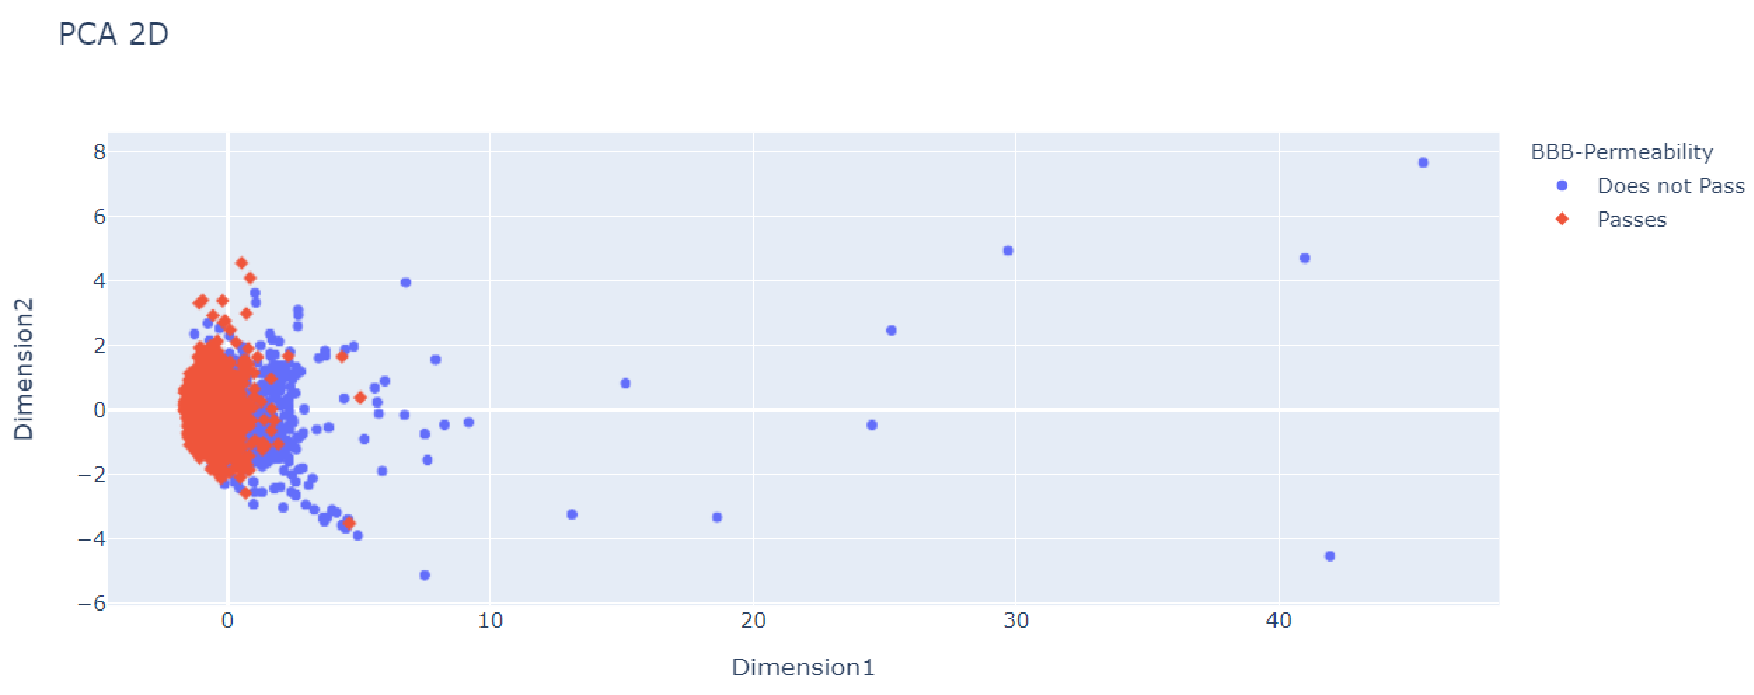
\includegraphics[width=1.0\linewidth]{images/PCA.pdf}    

    \caption{Principal component analysis plot after projecting the data set to a two-dimensional space.}

    \label{fig:PCA} 
\end{figure}


\subsection{Chemical Descriptors Ranges}
\label{subsec:CD_Ranges}

To explore our chemical descriptor data ranges, we decided to create violin plots combined with box plots.

It should be noted that the following discussion will explore the distributions found in our specific data set, a sample of drugs and compounds which may or may not be representative of the whole population of drugs and compounds that can penetrate the blood-brain barrier and of those that cannot.

Molecular Weight (MW) distribution, showcased by Figure \ref{fig:MW_Ranges}, showed that the greater number of drugs and compounds that could pass the blood-brain barrier had a MW in the range of 237.2-377.5. Whereas the majority of drugs and compounds that could not pass the blood-brain barrier had a MW in the range 318.4-539.6. A note should be made of the very large outliers appearing in the BBB- drugs and compounds, with a notable example having a MW of 7127. It appears that a smaller MW is preferable for BBB penetration. However, this is not always the case, as we can see BBB- drugs and compounds with a very low MW.

\begin{figure}[!ht]
    \centering
    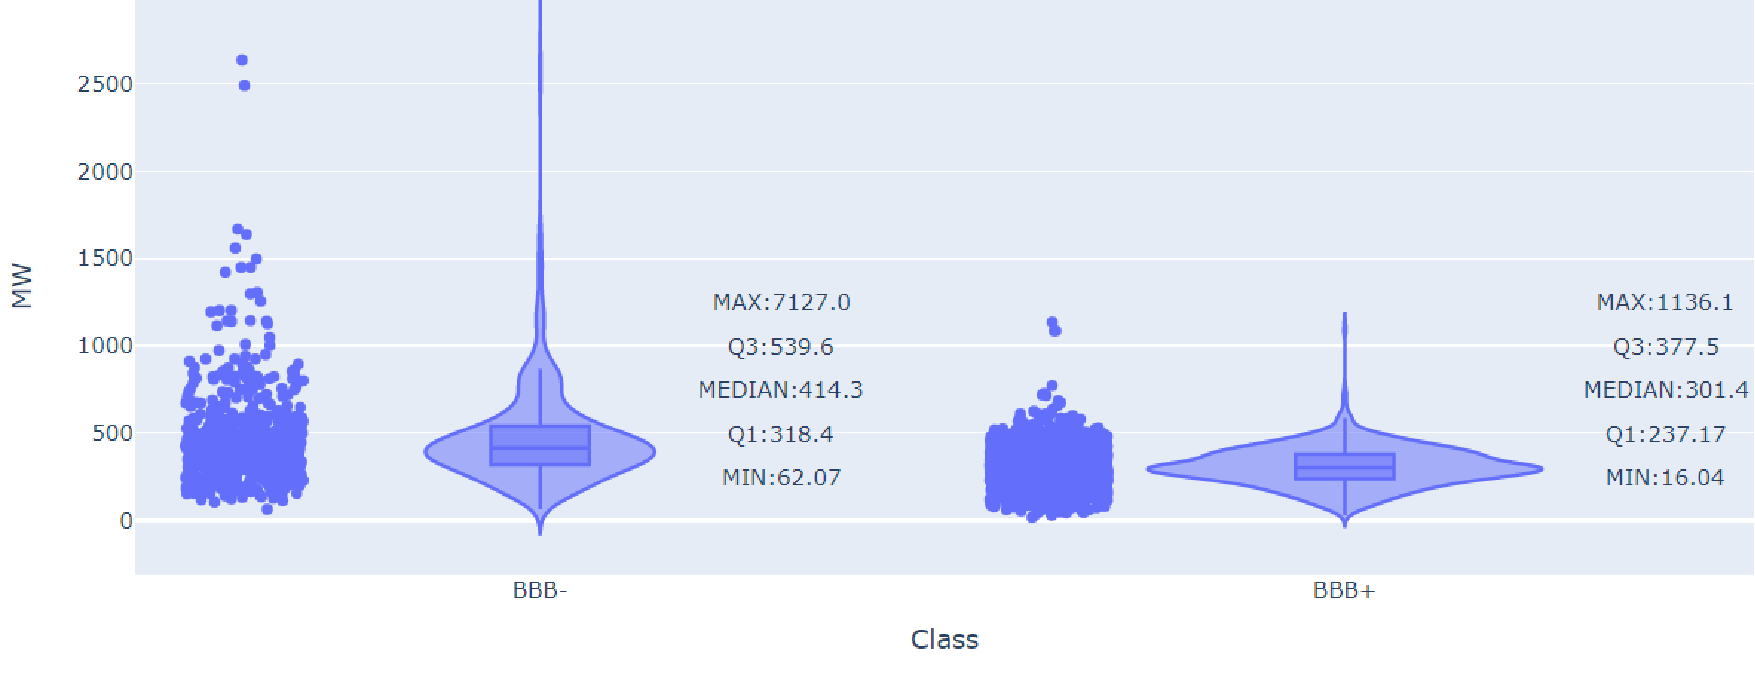
\includegraphics[width=0.9\linewidth]{images/MW Ranges.pdf}    

    \caption{Violin plots for the distribution of molecular weight (MW) values of each class}

    \label{fig:MW_Ranges} 
\end{figure}

Topological polar surface area (TPSA) distribution, showcased by Figure \ref{fig:TPSA_Ranges}, showed that the greater number of drugs and compounds that could pass the blood-brain barrier had a TPSA in the range of 32.3-74.6. Whereas the majority of drugs and compounds that could not pass the blood-brain barrier had a TPSA in the range 79.3-197. Again we can see some very large outliers in the BBB- drugs and compounds, with a notable example having a TPSA of 2860. Just as in the case of MW, it appears that a smaller TPSA is preferable.

\begin{figure}[!ht]
    \centering
    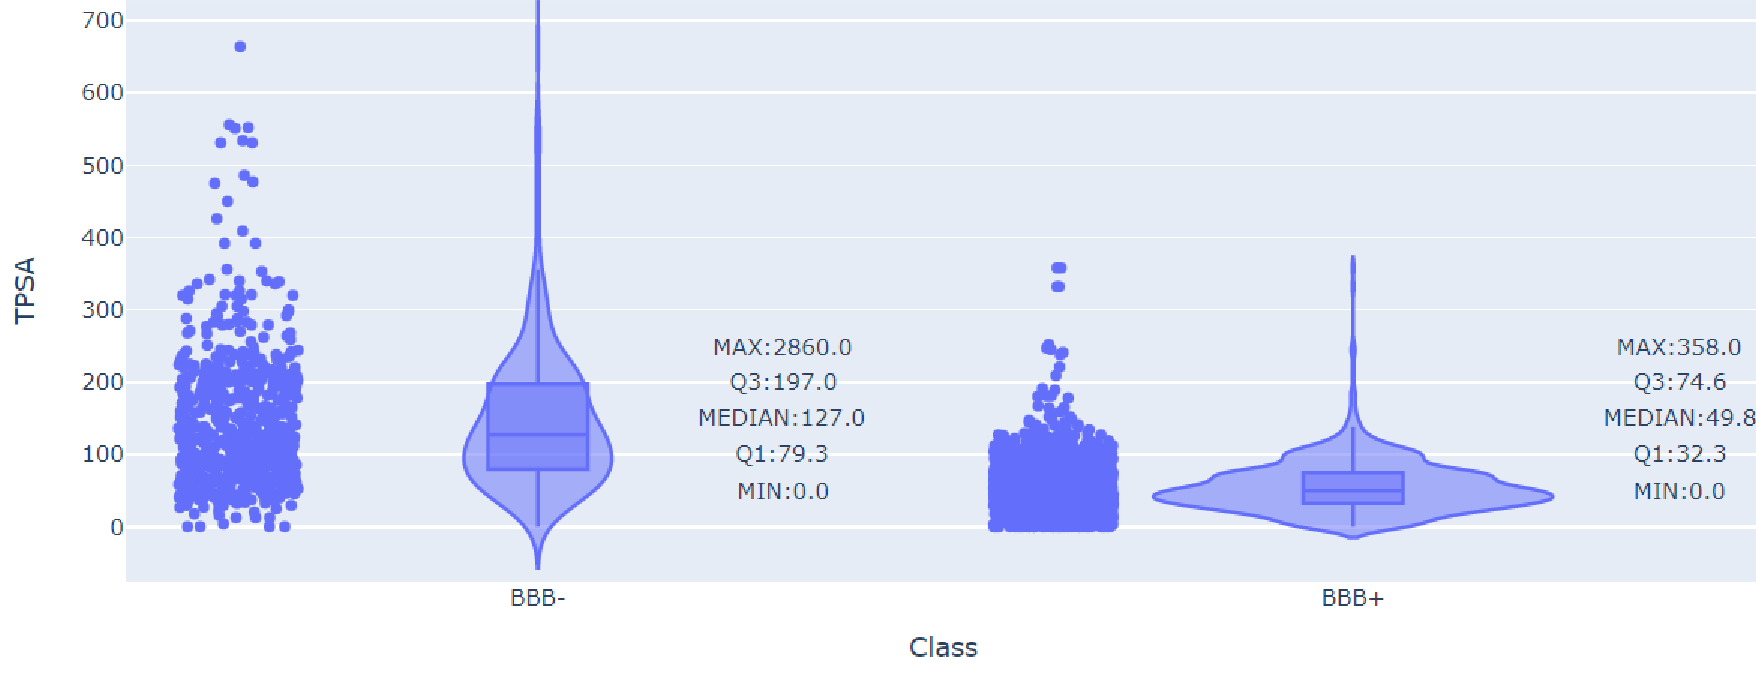
\includegraphics[width=0.9\linewidth]{images/TPSA Ranges.pdf}    

    \caption{Violin plots for the distribution of topological polar surface area (TPSA) values of each class}

    \label{fig:TPSA_Ranges} 
\end{figure}

Octanol-water partition coefficient (XLogP) distribution, showcased by Figure \ref{fig:XLogP_Ranges}, showed that the greater number of drugs and compounds that could pass the blood-brain barrier had an XLogP in the range of 1.6-3.8. Whereas the majority of drugs and compounds that could not pass the blood-brain barrier had an XLogP in the range -0.5-2.9. Again we can see some significant outliers in the BBB- drugs and compounds, with a notable example having an XLogP of -37.7. It seems that a small but positive XLogP is preferable.

\begin{figure}[!ht]
    \centering
    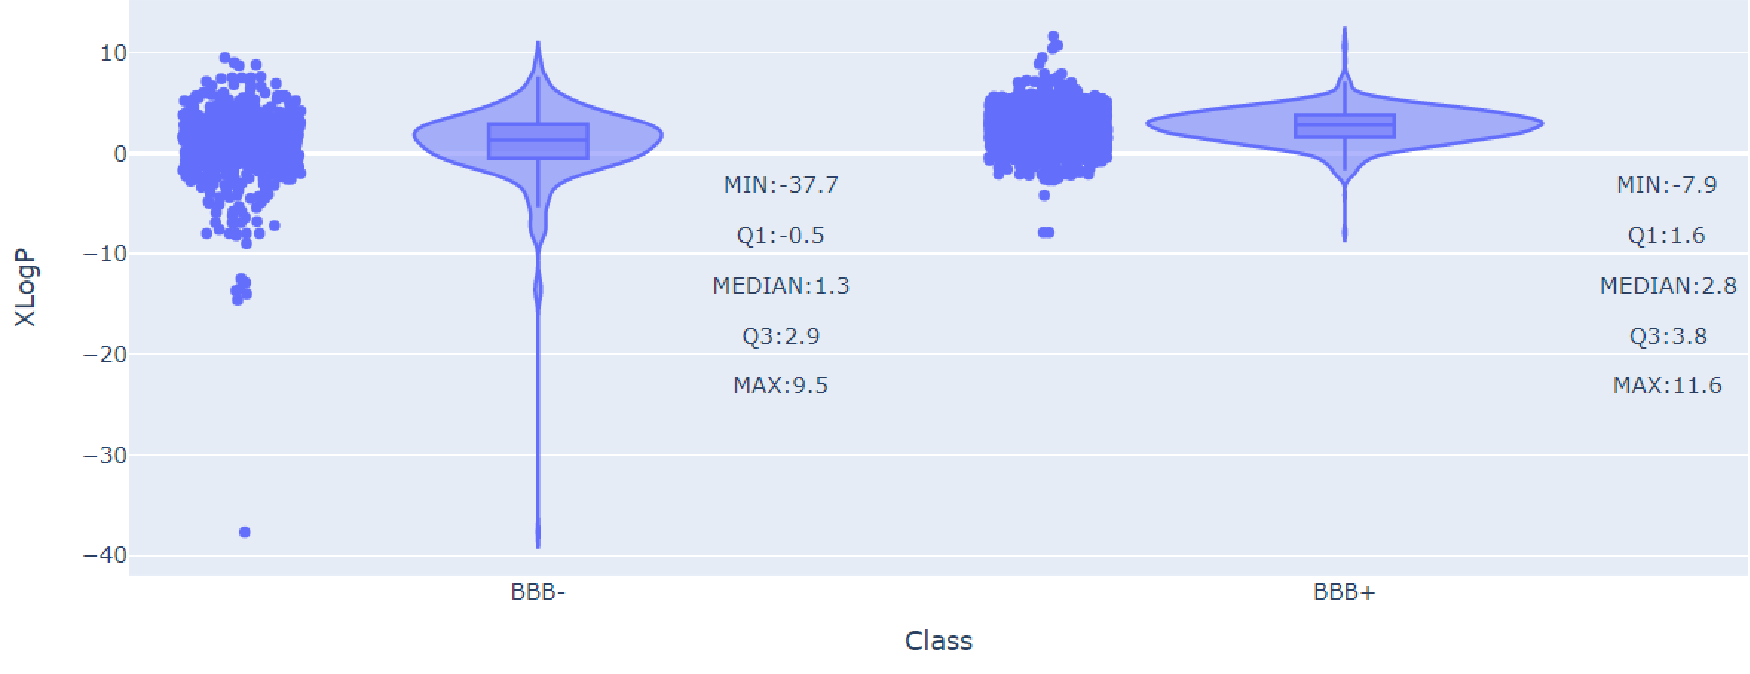
\includegraphics[width=0.9\linewidth]{images/XLogP Ranges.pdf}    

    \caption{Violin plots for the distribution of octanol-water partition coefficient (XLogP) values of each class}

    \label{fig:XLogP_Ranges} 
\end{figure}

Hydrogen-bond donors (NHD) distribution, showcased by Figure \ref{fig:NHD_Ranges}, showed that the greater number of drugs and compounds that could pass the blood-brain barrier had an NHD in the range of 0-2. Whereas the majority of drugs and compounds that could not pass the blood-brain barrier had an NHD in the range 2-4. Again we can see some significant outliers in the BBB- drugs and compounds, with a notable example having an NHD of 77. It seems that a smaller NHD is preferable.

\begin{figure}[!ht]
    \centering
    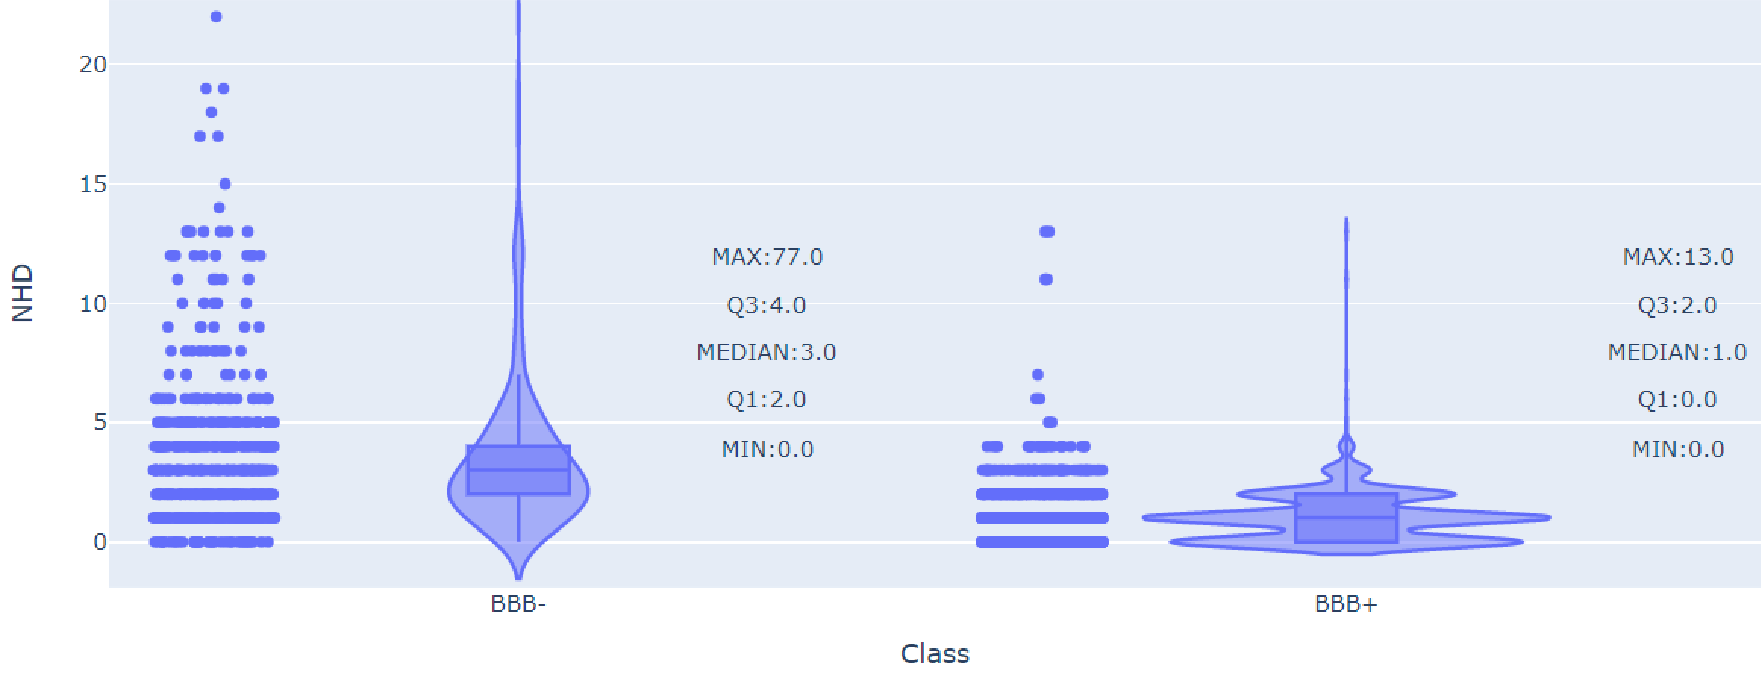
\includegraphics[width=0.9\linewidth]{images/NHD Ranges.pdf}    

    \caption{Violin plots for the distribution of the number of hydrogen-bond donors (NHD) of each class}

    \label{fig:NHD_Ranges} 
\end{figure}

Hydrogen-bond acceptors (NHA) distribution, showcased by Figure \ref{fig:NHA_Ranges}, showed that the greater number of drugs and compounds that could pass the blood-brain barrier had an NHA in the range of 2-5. Whereas the majority of drugs and compounds that could not pass the blood-brain barrier had an NHD in the range 5-11. Again we can see some significant outliers in the BBB- drugs and compounds, with a notable example having an NHA of 167. Just as in the case of NHD, it appears that a smaller NHA is preferable.

\newpage

\begin{figure}[!ht]
    \centering
    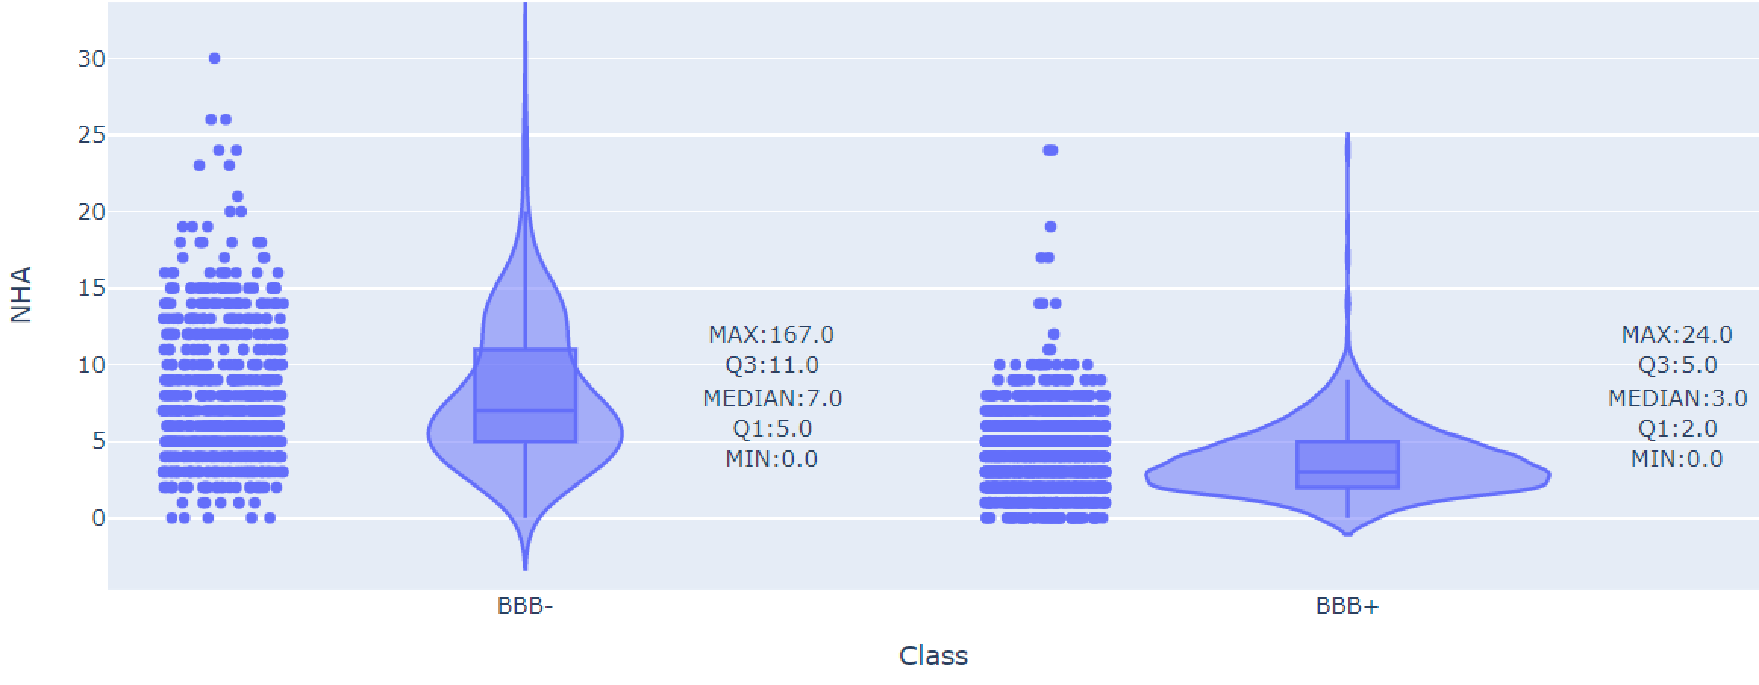
\includegraphics[width=0.9\linewidth]{images/NHA Ranges.pdf}    

    \caption{Violin plots for the distribution of the number of hydrogen-bond acceptors (NHA) of each class}

    \label{fig:NHA_Ranges} 
\end{figure}

The number of rotatable bonds (NRB) distribution, showcased by Figure \ref{fig:NRB_Ranges}, showed that the greater number of drugs and compounds that could pass the blood-brain barrier had an NRB in the range of 2-6. Whereas the majority of drugs and compounds that could not pass the blood-brain barrier had an NHD in the range 3-8. Again we can see some significant outliers in the BBB- drugs and compounds, with a notable example having an NRB of 178. Just as in the case of NHD and NHA, it appears that a smaller NRB is preferable. However, it is a bit unclear due to a considerable overlap between the two classes.

\begin{figure}[!ht]
    \centering
    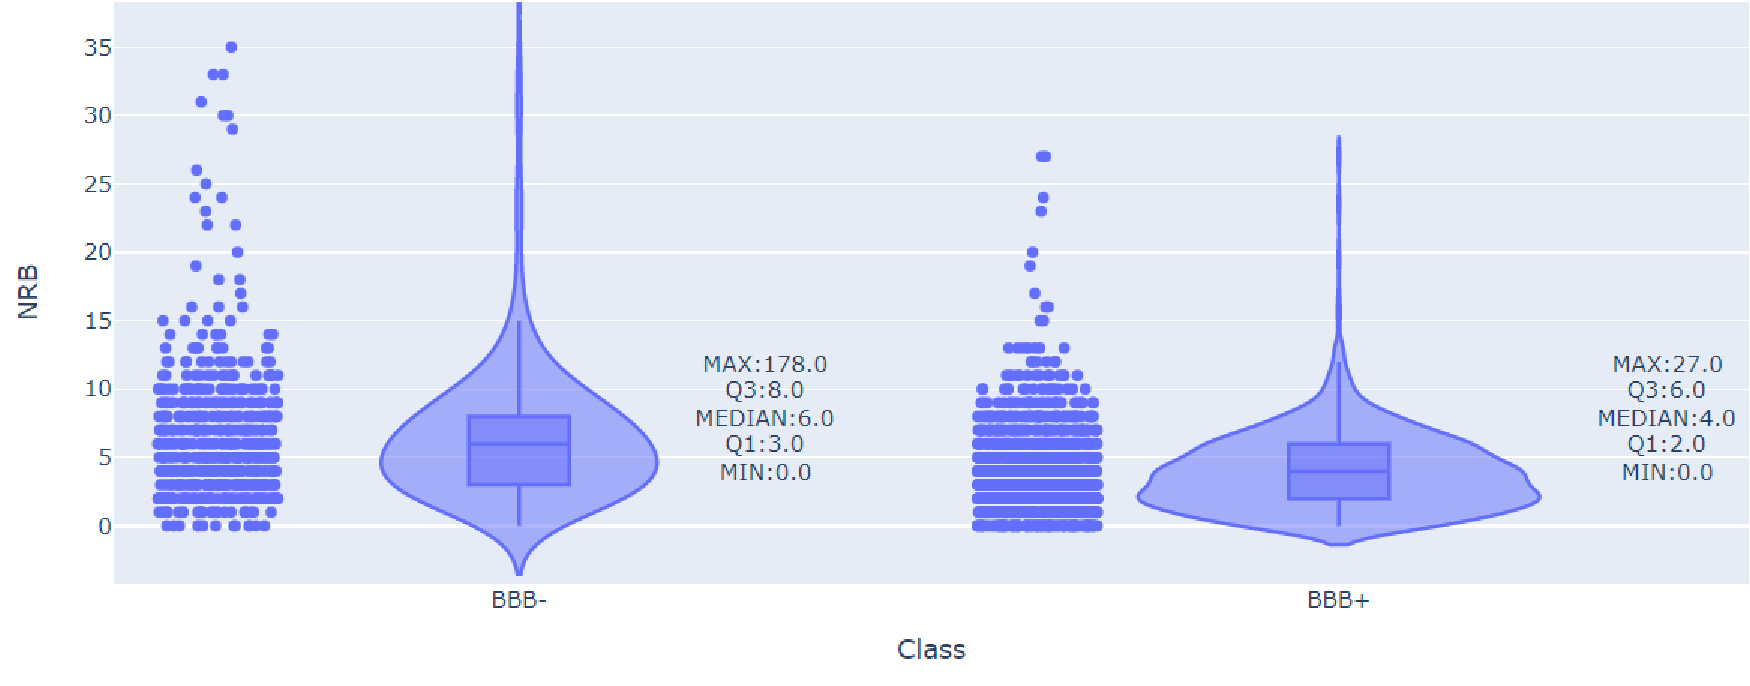
\includegraphics[width=0.9\linewidth]{images/NRB Ranges.pdf}    

    \caption{Violin plots for the distribution of the number of rotatable bonds (NRB) of each class}

    \label{fig:NRB_Ranges} 
\end{figure}

\subsection{Important Side Effects \& Indications}

As we have previously discussed in Subsection \ref{subsec:Classification_Models}, RFECV was used to primarily reduce the large number of side effects and indications used by some classification models. 

Table \ref{tbl:Side_Effects} showcases all the different side effects deemed highly important by RFECV. Some of them, such as depressed levels of consciousness or a coma, naturally seem sensible choices as they seem directly connected to the central nervous system. However, others, such as dry skin or influenza, seem less so.

Table \ref{tbl:Indications} showcases all the different indications deemed highly important by RFECV. In our opinion, all indications returned seem sensible.

\begin{table}[!ht]
  \caption{Top side effects according to RFECV. *Please ignore the <NA> entries, these were used as padding when creating the table.}
  \label{tbl:Side_Effects}
  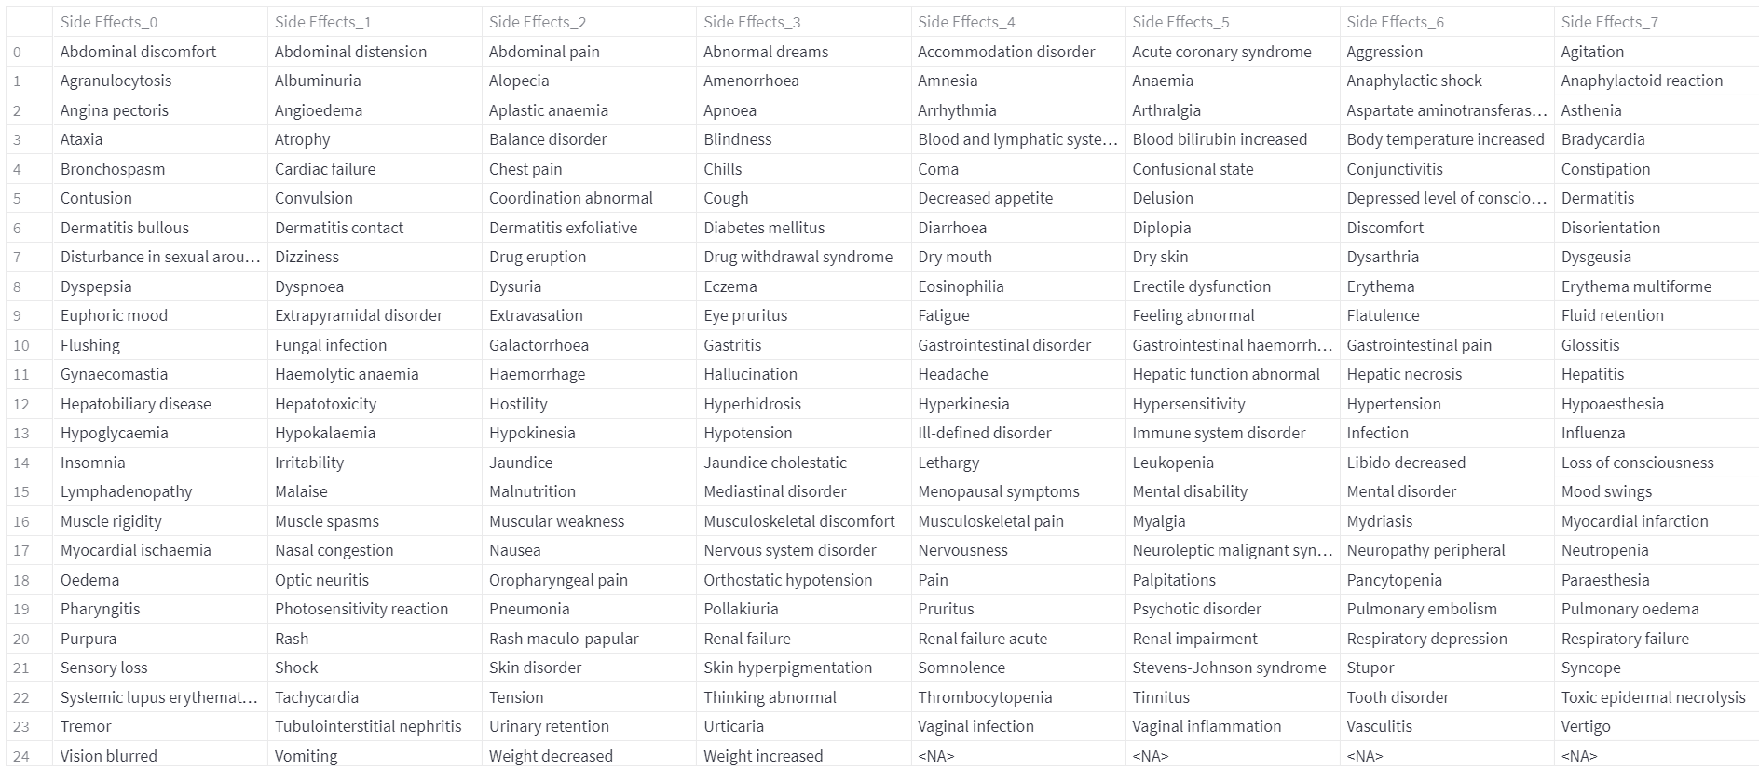
\includegraphics[width=1.0\linewidth]{images/Side Effects.pdf}
\end{table}

\begin{table}[!ht]
  \caption{Top indications according to RFECV.}
  \label{tbl:Indications}
  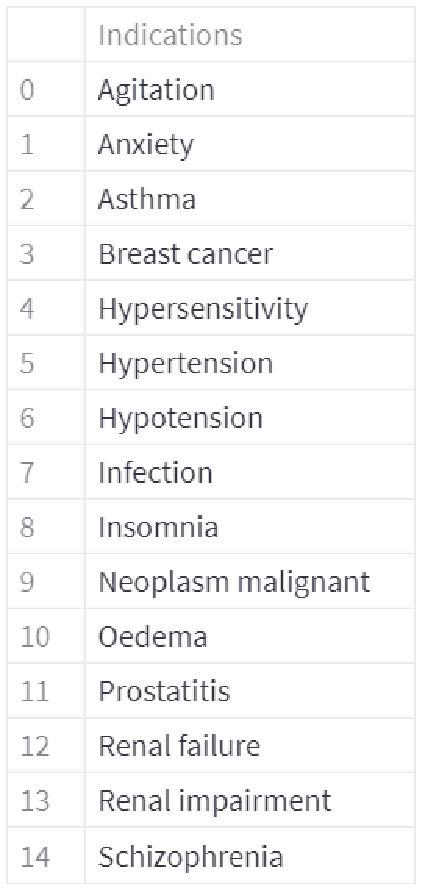
\includegraphics[width=0.2\linewidth]{images/Indications.pdf}
\end{table}


\section{Models Performance}

This section discusses the robustness and predictive performances of the different trained models and makes some comparisons.

\subsection{Classification Models Utilising Chemical Descriptors}
\label{subsec:Classification_CD}

Tables \ref{tbl:Classification_CD_Training} and \ref{tbl:Classification_CD_Testing} showcase the training and testing scores of all our classification models that only used chemical descriptors as their features. All of our models appear robust, with a permutation test p-value < 0.05, making them statistically significant. 

Even though six models were produced, excluding the Dummy Classifier, which is only used as a baseline, we would not recommend the use of the Logistic Regression and Support Vector Classification models. These models are only slightly better than the Dummy Classifier and have a very low MCC score, making them just marginally better than a coin flip.

Our best model seems to be the Random Forest Classifier, outperforming all the other models in every metric. A very close second would be the K-Nearest Neighbour Classifier.

\begin{table}
  \caption{Training performance of classification models with chemical descriptors used as features.}
  \label{tbl:Classification_CD_Training}
  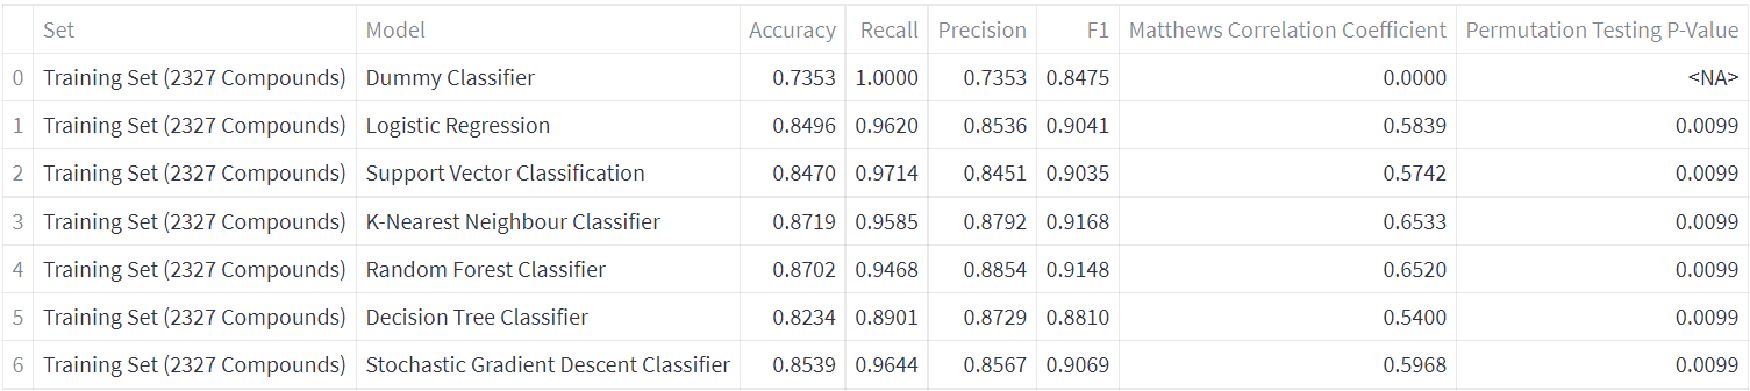
\includegraphics[width=1.0\linewidth]{images/Classification CD Training.pdf}
\end{table}

\begin{table}
  \caption{Testing performance of classification models with chemical descriptors used as features.}
  \label{tbl:Classification_CD_Testing}
  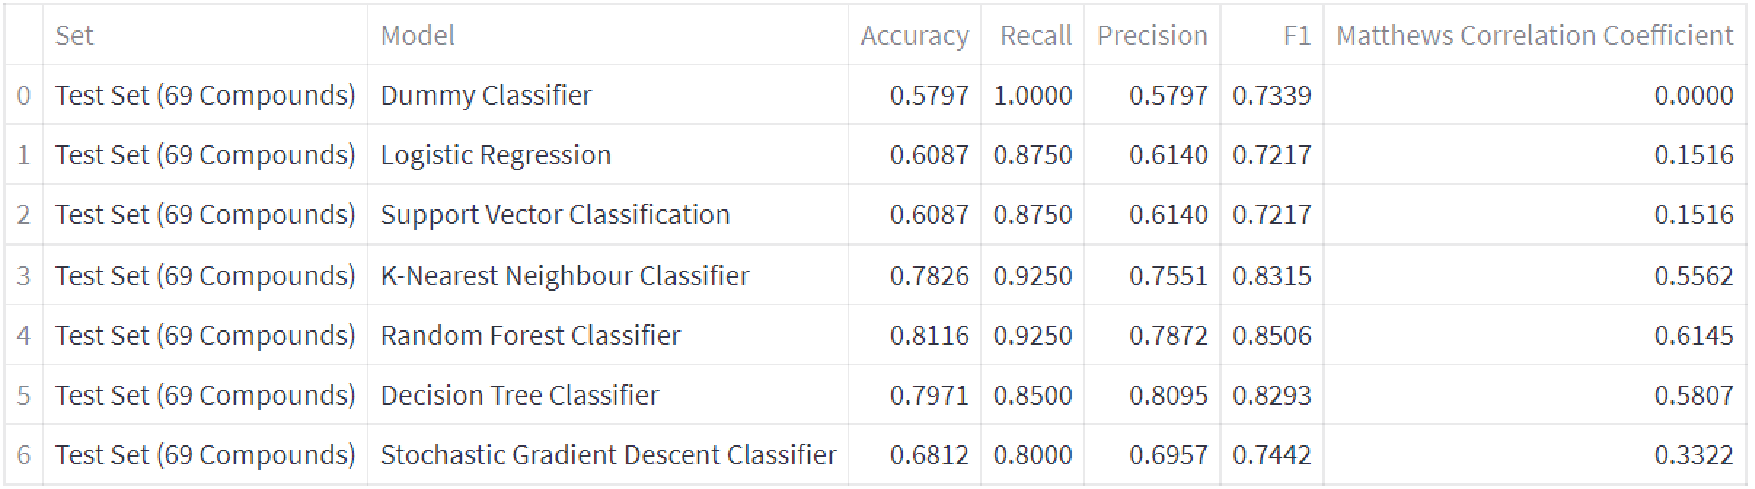
\includegraphics[width=1.0\linewidth]{images/Classification CD Testing.pdf}
\end{table}

\subsection{Classification Models Utilising Chemical Descriptors, Side Effects \& Indications}

Tables \ref{tbl:Classification_CD_SE_I_Training} and \ref{tbl:Classification_CD_SE_I_Testing} showcase the training and testing scores of all our classification models that used chemical descriptors, side effects and indications as their features. All of our models appear to be robust, with a permutation test p-value < 0.05, making them statistically significant. 

The addition of side effects and indications to the chemical descriptors appears to have substantially improved the performance of almost all models, except in the case of the Decision Tree Classifier, where its performance decreased.

Again, our best model seems to be the Random Forest Classifier, outperforming all the other models in every metric. A very close second would be the K-Nearest Neighbour Classifier.

\begin{table}[!ht]
  \caption{Training performance of classification models with chemical descriptors, side effects and indication used as features.}
  \label{tbl:Classification_CD_SE_I_Training}
  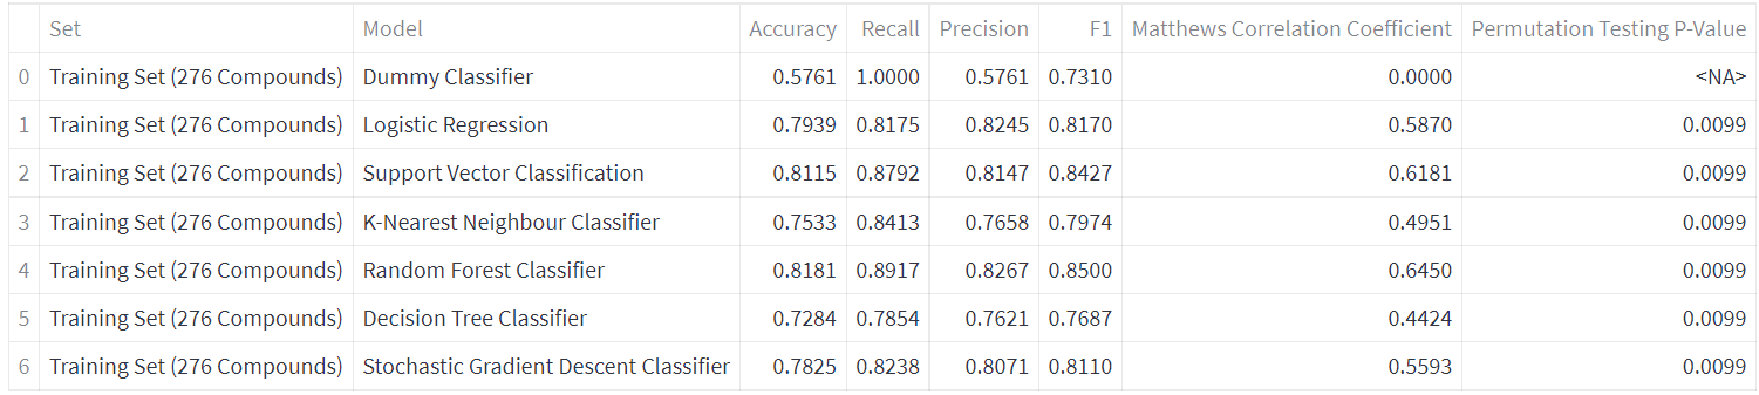
\includegraphics[width=1.0\linewidth]{images/Classification CD SE I Training.pdf}
\end{table}

\newpage

\begin{table}[!ht]
  \caption{Testing performance of classification models with chemical descriptors, side effects and indication used as features.}
  \label{tbl:Classification_CD_SE_I_Testing}
  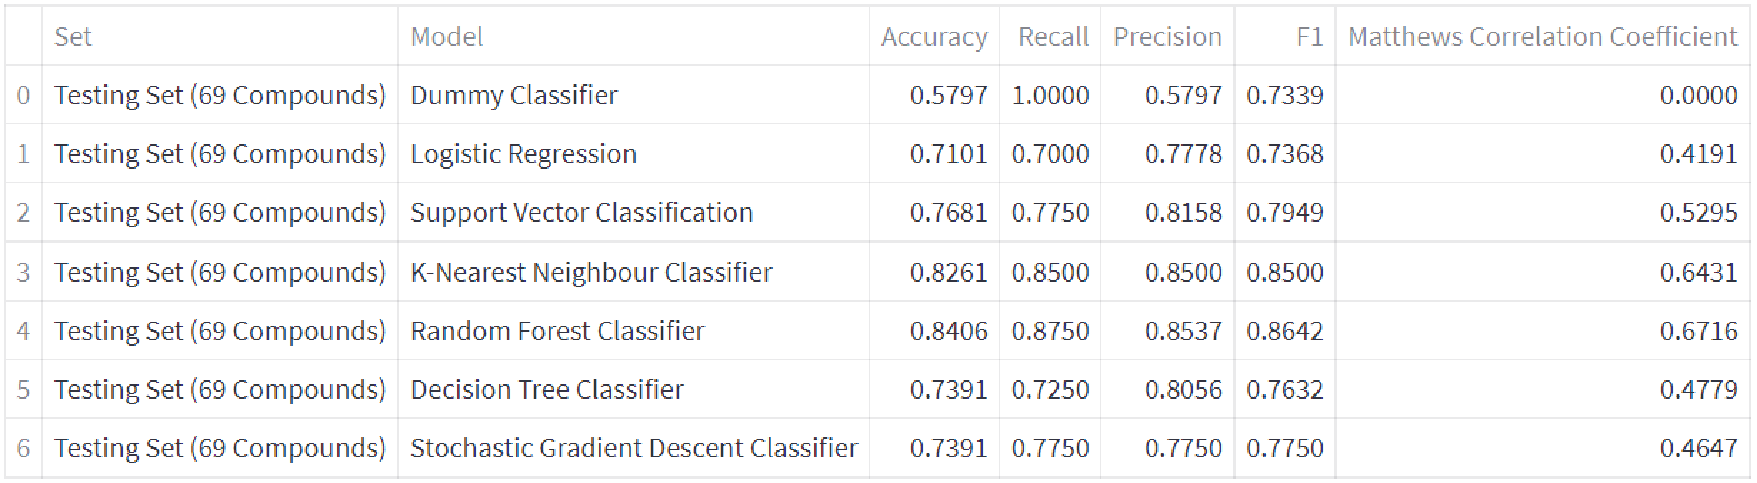
\includegraphics[width=1.0\linewidth]{images/Classification CD SE I Testing.pdf}
\end{table}

\subsection{Regression Models Utilising Chemical Descriptors}

Tables \ref{tbl:Regression_CD_Training} and \ref{tbl:Regression_CD_Testing} showcase the training and testing scores of all our regression models that only used chemical descriptors as their features. All of our models, except the Decision Tree Regressor, appear to be robust, with a permutation test p-value < 0.05, making them statistically significant. 

Our best model seems to be the Support Vector Regression, outperforming all the other models in every metric.

\begin{table}[!ht]
  \caption{Training performance of regression models with chemical descriptors used as features.}
  \label{tbl:Regression_CD_Training}
  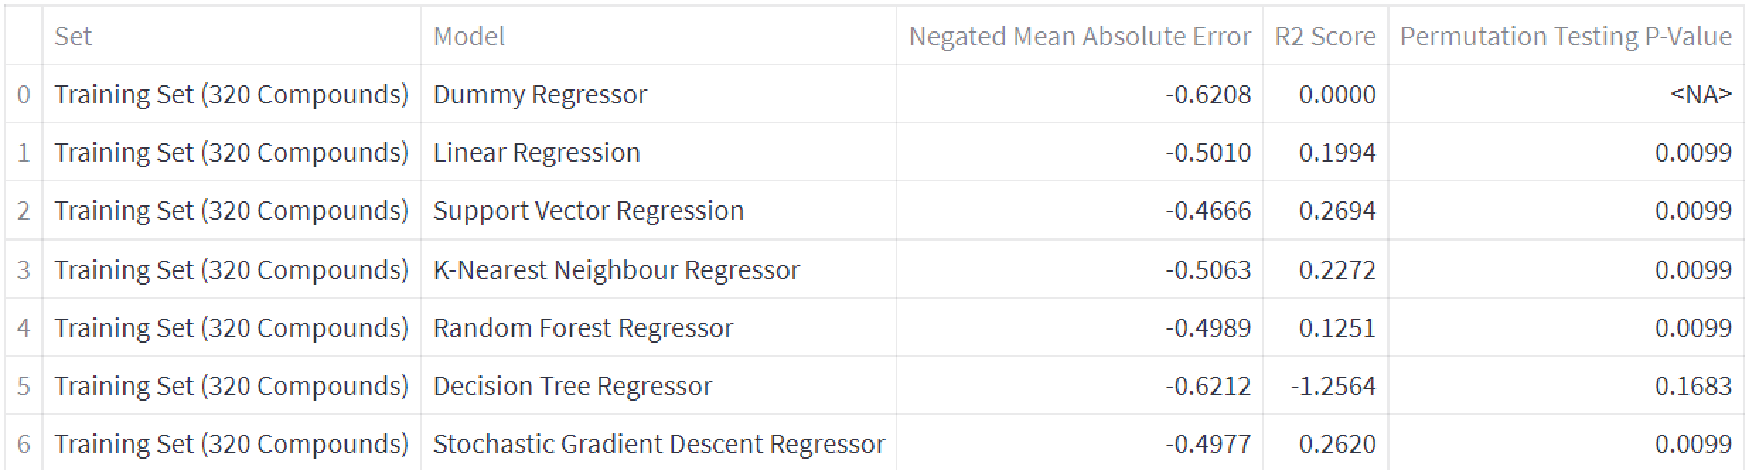
\includegraphics[width=1.0\linewidth]{images/Regression CD Training.pdf}
\end{table}

\begin{table}[!ht]
  \caption{Testing performance of regression models with chemical descriptors used as features.}
  \label{tbl:Regression_CD_Testing}
  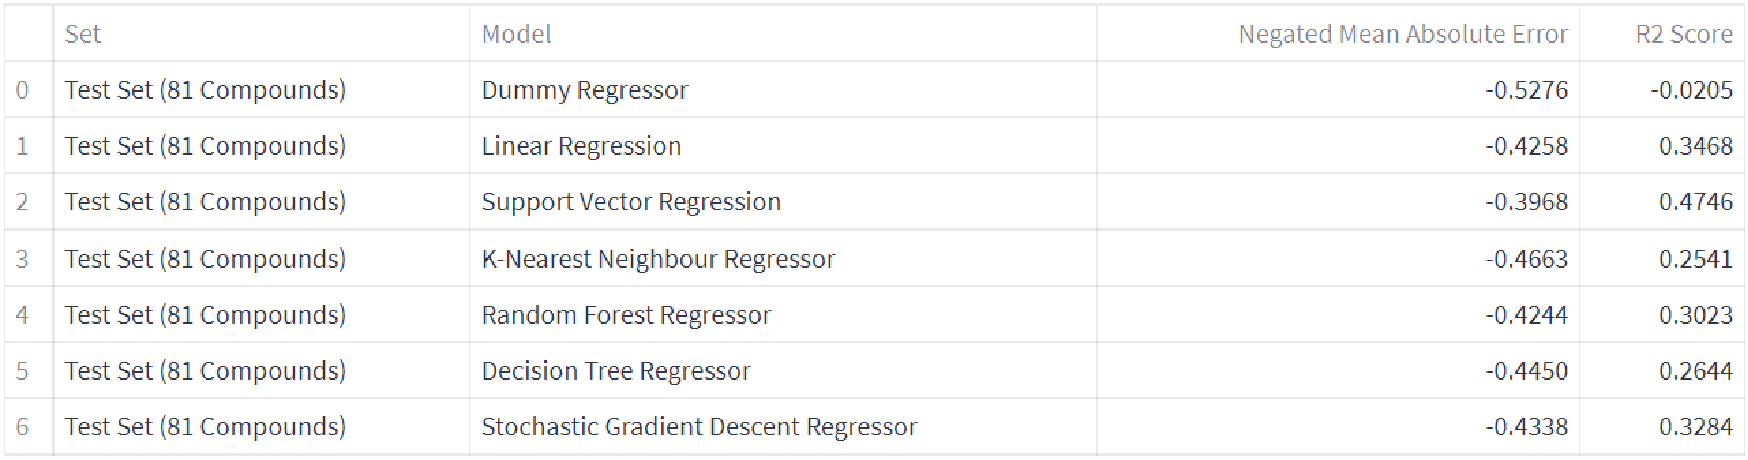
\includegraphics[width=1.0\linewidth]{images/Regression CD Testing.pdf}
\end{table}

\section{Project Evaluation}

All objectives specified in Section \ref{sec:Objectives} were successfully achieved. 

We managed to create a substantial data set that was used to create both classification and regression models using a very small number of chemical descriptors, further confirming the conclusions reached by \citet{Zhao2007, Saber2020} that models predicting the blood-brain barrier permeability of drugs and compounds can be built using a minimal number of hydrogen-bonding chemical descriptors. All of our models, except for a single one, were statistically significant however some were only marginally better than a coin flip as discussed in Subsection \ref{subsec:Classification_CD}

The project also managed to validate the conclusion reached by \cite{Gao2017} that the addition of side effects and indications to chemical descriptors substantially improved the predictive performance of models. All but one of our classification models' predictive performances improved by adding side effects and indications, even though we used a different technique and a smaller number of chemical descriptors. Our Random Forest Classifier even achieved somewhat similar performance to the Support Vector Machine trained by \citet{Gao2017}, showcased by Table \ref{tbl:Gao_Model_Comparison}.
%==================================================================================================================================
\chapter{Conclusion}    
%Summarise the whole project for a lazy reader who didn't read the %rest (e.g. a prize-awarding committee). This chapter should be short %in most dissertations; maybe one to three pages.
%\section{Guidance}
%\begin{itemize}
%    \item
%        Summarise briefly and fairly.
%    \item
%        You should be addressing the general problem you introduced %in the
%        Introduction.        
%    \item
%        Include summary of concrete results (``the new compiler ran %2x
%        faster'')
%    \item
%        Indicate what future work could be done, but remember: %\textbf{you
%        won't get credit for things you haven't done}.
%\end{itemize}

This chapter summarises the project and discusses valuable lessons learned and any possible future work that could potentially improve upon our findings. 


\section{Summary}

The brain is surrounded by a semi-permeable boundary that prevents many pathogens from getting in. However, it can also stop many useful drugs from entering the brain. This is especially important when trying to deliver critical therapeutics, such as chemotherapy, to brain tumours. Therefore, accurate prediction of whether a drug will easily cross the blood-brain barrier is a valuable tool for developing and testing new drugs for various diseases.

This project aimed to gather publicly available data on drugs known to cross into the brain and those that cannot and place them into a new data set and then, using that new data set, train machine learning models that use a drug's or compound's chemical descriptors to predict whether it can pass into the brain or not.

A data set of 2396 publicly available compounds and drugs was gathered from various academic papers and medical APIs, subsets of which were used to train both classification and regression models. Various models were trained for both types of models using a tiny number of chemical descriptors, checked for robustness and evaluated using test sets and dummy models. In the case of classification models, these were further improved by including the available side effects and indications of each drug and compound. Unfortunately, this could not be replicated for the regression models due to the small size of available drugs having all the necessary information we required.

A Streamlit web application was then created to present a synopsis of our work and primarily showcase our models, allowing users to use them to make predictions. A strong emphasis was also placed on model interpretability, potentially helping users understand what led to a specific prediction by a model. A strong chemical or medical knowledge is not necessarily needed, but it would definitely be a plus. 

Our best classification model with just chemical descriptors used as features was the Random Forest Classifier which achieved an F1 score of 0.8506, an Accuracy of 0.8116, a Recall score of 0.9250, a Precision score of 0.7872 and a Matthews Correlation Coefficient of 0.6145.

Our best classification model with chemical descriptors and a selection of side effects and indications as features was again the Random Forest Classifier, which achieved an F1 score of 0.8642, an Accuracy of 0.8406, a Recall score of 0.8750, a Precision score of 0.8537 and a Matthews Correlation Coefficient of 0.6716.

Our best regression model with chemical descriptors used as features was the Support Vector Regression model, which achieved an R2 score of 0.4746, and a Negated Mean Absolute Error of -0.3968.

The created models can be used efficiently to predict the blood-brain permeability of thousands of already existing or new drugs and compounds. However, these predictions should be taken as guidelines for further research, possibly even experimental trials in order to confirm them, and not as absolutes, as no model can be perfect.

\section{Reflection}

This project allowed us to work in-depth with previously unfamiliar concepts, mainly bioinformatics and machine learning, and to learn multiple new skills, best practices, and techniques that we can build upon in the future. 

Looking back at the project, we should have definitely used a common testing set with one of the background papers in Chapter \ref{ch:Background} so we could directly compare our models' performance and to see if we achieved a better predictive performance or not, expand our data set even more, and spent more time and energy analysing the errors of our models. However, overall we believe the project to be a success, achieving all of its specified objectives in a professional and responsible manner.

\section{Future work}

Even though it could be argued that the project was reasonably successful, a few areas of improvement could be explored further in the future. 

The data set could be expanded with the help of professionals with chemical and medical knowledge that could potentially point out any mislabelled entries, which could then be used to retrain the models or create new ones, even potentially utilising deep learning to produce even better models with greater predictive performances.

The already trained models could be improved by analysing their blind spots, the chemical areas of drugs and compounds that are consistently misclassified or produce a high error value. Some preliminary error analysis of the predictions made by our models found what appear to be groupings, suggesting that there is some pattern that could be looked at in more detail. These systematic weaknesses could be negated by further exploring the errors, but some in-depth chemical knowledge would be required, which we did not have during the project's life-cycle.

%==================================================================================================================================
%
% 
%==================================================================================================================================
%==================================================================================================================================
%   BIBLIOGRAPHY   

% The bibliography style is agsm (Harvard)
% The bibliography always appears last, after the appendices.

\bibliographystyle{agsm}

% Force the bibliography not to be numbered
\renewcommand{\thechapter}{0} 
\bibliography{l4proj}

\end{document}
